\documentclass[utf8x]{ctexart}
\usepackage{setspace}
\usepackage{url}
\onehalfspacing
\usepackage{amsmath,amssymb,amsfonts,amsthm,mathtools}
\usepackage[english]{babel}
\usepackage[T1]{fontenc}
\usepackage{lmodern}
\usepackage{dsfont}
\usepackage{bbm}
\usepackage[round]{natbib}
\usepackage{color} 
\usepackage[defaultlines=2,all]{nowidow}
\usepackage{caption}
\usepackage[labelformat=simple]{subcaption}
\usepackage{makecell}
\renewcommand\thesubfigure{(\alph{subfigure})}

\setlength\parindent{0pt}
\setlength{\parskip}{6pt plus 1pt minus 1pt}

\newcommand{\red}{\textcolor{red}}


\begin{document}

\begin{titlepage}
  \centering
  {\scshape\LARGE National Taiwan University \par}
  \vspace{1cm}
  {\scshape\Large Financial Technology \par}
  \vspace{2cm}
  {\huge\bfseries Project 1: Credit Card Fraud Detection\par}
  \vspace{2cm}
  {\Large Lecturer:\\
    Che Lin (林澤) \par}
  \vspace{1cm}
  {\Large Author: Tadeo Hepperle, Student ID: A11922105 \par}
  \vfill
  {\large \today\par}
\end{titlepage}


\tableofcontents

\cleardoublepage

\section{Introduction}

In this project we use a dataset from Kaggle "Credit Card Fraud Detection" to predict fraudulent spendings on credit cards, given a range of features. For this task, we will compare classical machine learning models like logistic regression, support vector machines and random forests with deep neural networks and evaluate their performance.

\subsection{Description of the data}

The dataset was originally from Kaggle, named "Credit Card Fraud Detection" and contains 31 variables, grouped into 30 features and one class label. Two of these features are the time the transaction took place and the amount spent. The 28 remaining features were obtained by performing a principal component analysis on a larger dataset. The classlabel is either 0 (normal) or 1 (fraudulent) for each record. The entire data consists of 99999 independent transaction records. Of those only 223 are fraudulent, which amounts to only 0.22\% and makes the data extremely unbalanced.

\subsection{Description of methods}

Besides deep neural networks, we also take a brief look at logistic regression, support vector machines and random forest models.

\subsubsection{Logistic Regression}
In Logistic regression we try to predict a binary response by using an array of numeric features. The model formula looks like this:

\[ P(y=1) =  \frac{exp(\beta_0 + \beta_1x_1 + \dots + \beta_kx_k)}{1 + exp(\beta_0 + \beta_1x_1 + \dots + \beta_kx_k)}\]

where $P(y=1)$ represents the probability of class 1 (fraud in our case) and the $x_1, \dots, x_k$ represent $k$ predictors. The probability of the other class ($P(y=0)$) is therefore $1-P(y=1)$.
Because the derivative of the logistic function is never 0 there is no closed form solution and methods like gradient descent need to be used for optimization. However if the data is linearly separable, these methods will never converge and will result in an "infinitely steep" probability curve.

\subsubsection{Support Vector Machines}

Support Vector Machines (SVM) aim to find a hyperplane that linearly seperates the data linearly into 2 homogeneous halfspaces. Because this is not always possible, two tricks can be applied. First, it is useful to use a soft margin instead of a hard one which allows some points of the wrong class to lie in the half space of the other class as long as they are still pretty close to the hyperplane. In some cases, like noisy data this can even give better classification results in cases where a hard margin could perfectly seperate the two classes. The second "Trick" that can be used to make Support Vector machines more useful is to use a certain kernel function to transform the input features to a different space domain. This can make even originally not linearly seperable data, seperable if the right transformations are used. In this project, we will not experiment with any kernel functions.

\subsubsection{Random Forest Classifier}

Random Forest is an ensemble method. That means it combines the power of an array of weak learners that on their own would perform poorly. Typically decision trees are used as the weak classifier, hence the name random "Forest". There are multiple ideas, how to let the individual trees learn and how to combine them. in Bootstrapping for example, we let each tree learn on a bootstrapping sample of the original data and later take a majority vote among all trees as the final decision. The bootstrapping sample is produced by randomly sampling objects from the data n times with put backs (where $n$ is the number of objects in total). The sample is different for every tree and can therefore allow the trees to learn different aspects of the data. The problem with this approach is, that the bootstrapping samples are still highly correlated. Random Forest aims to solve this, by further diversifying and restricting what data can be used by each tree during learning. The idea is simple: At each split to be made in a decision tree, not all features are considered, but only a subset of features is allowed to be used to make the split. Typically for $k$ features, $\sqrt{k}$ randomly selected features are allowed in each split. This increases the variance among weak learners and can lead to classification improvements.

\section{Results}

With an 80-20 train-test split of the data, 3 models were trained: Logistic Regression, Support Vector Machine and Random Forest Classifier.

\subsection{Confusion Matrices and Classification Metrics}
As Figure~\ref{fig:confusion1} shows, all models are pretty good at classifying the non-fraud cases as non-fraud, which is non-surprising since these comprise the overwhelming majority of the training data.
Taking a look at the classification metrics in Table~\ref{tab:metrics1} we can see that the SVM is overall performing best, also with highest accuracy. To judge the performance, I would use the F1-score as it provides a good middle ground between precision and recall, in both of which high values are desired. I think the F1 metric is most suitable on this dataset because it is not affected by the very imbalanced distribution of fraud vs. non-fraud cases in the data. The amount of True Negatives is very high in all classifiers used and the F1 score is not influenced by the amount of true negatives at all, which is a good thing in our case. Surprisingly Logistic Regression and Random Forest have the same performance.

\begin{figure}[htb]
  \centering
  \begin{subfigure}[b]{0.32\textwidth}
    \centering
    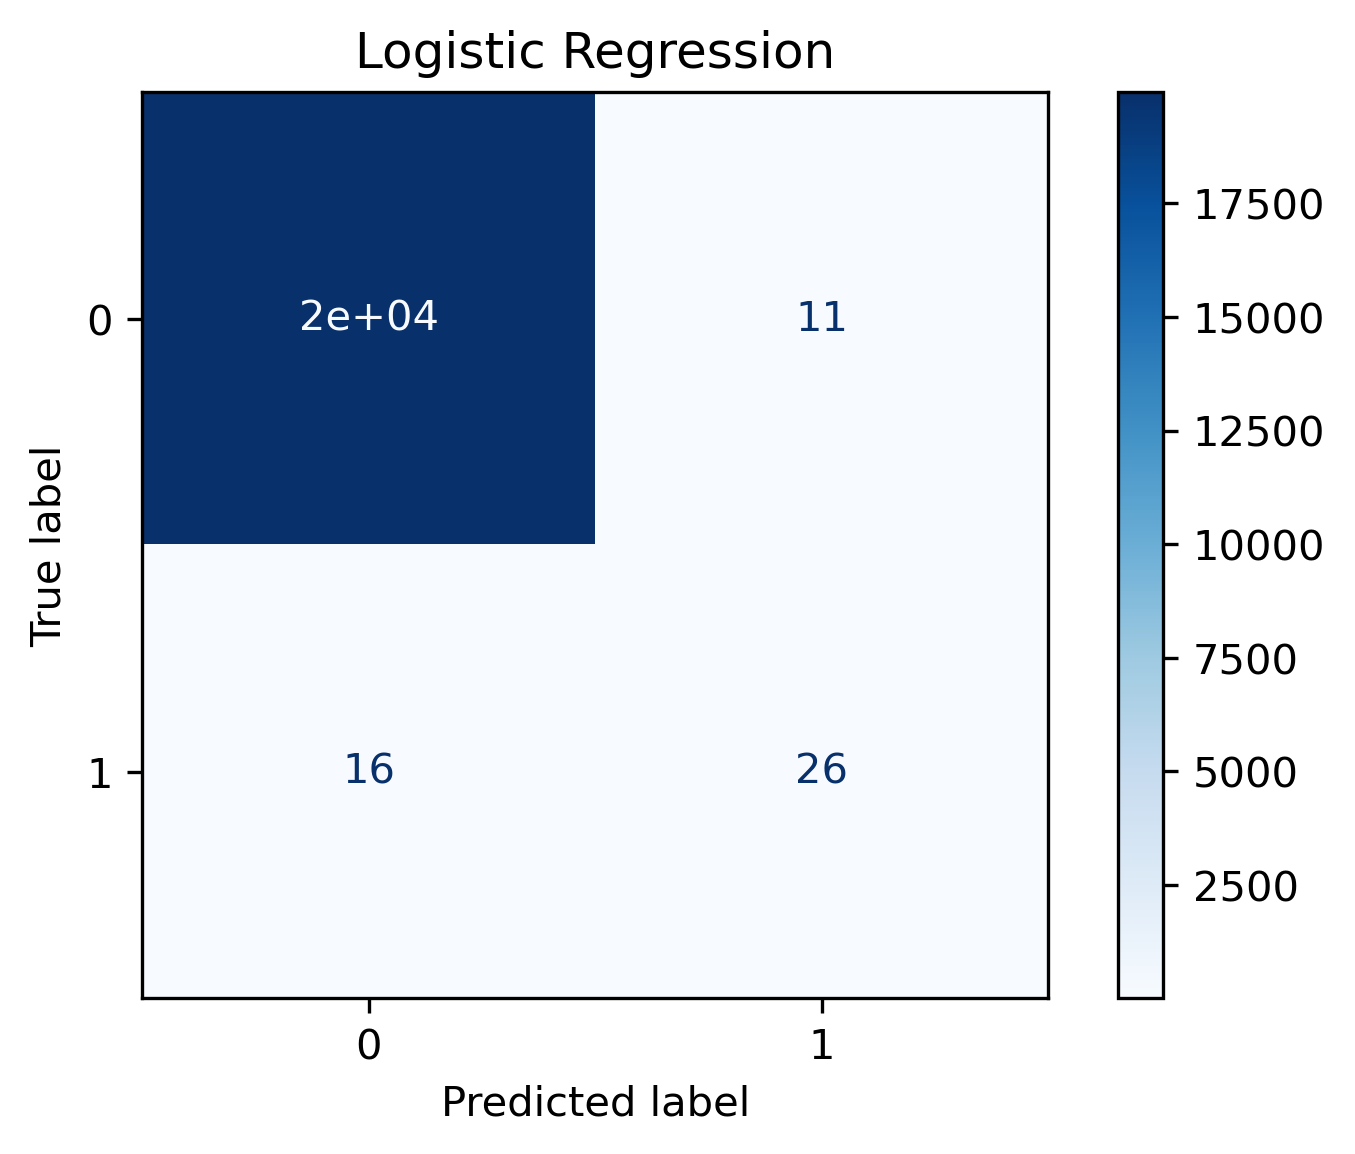
\includegraphics[width=\textwidth]{./images/reg_conf1.png}
    \label{fig:qqplotreszprice}
  \end{subfigure}
  \begin{subfigure}[b]{0.32\textwidth}
    \centering
    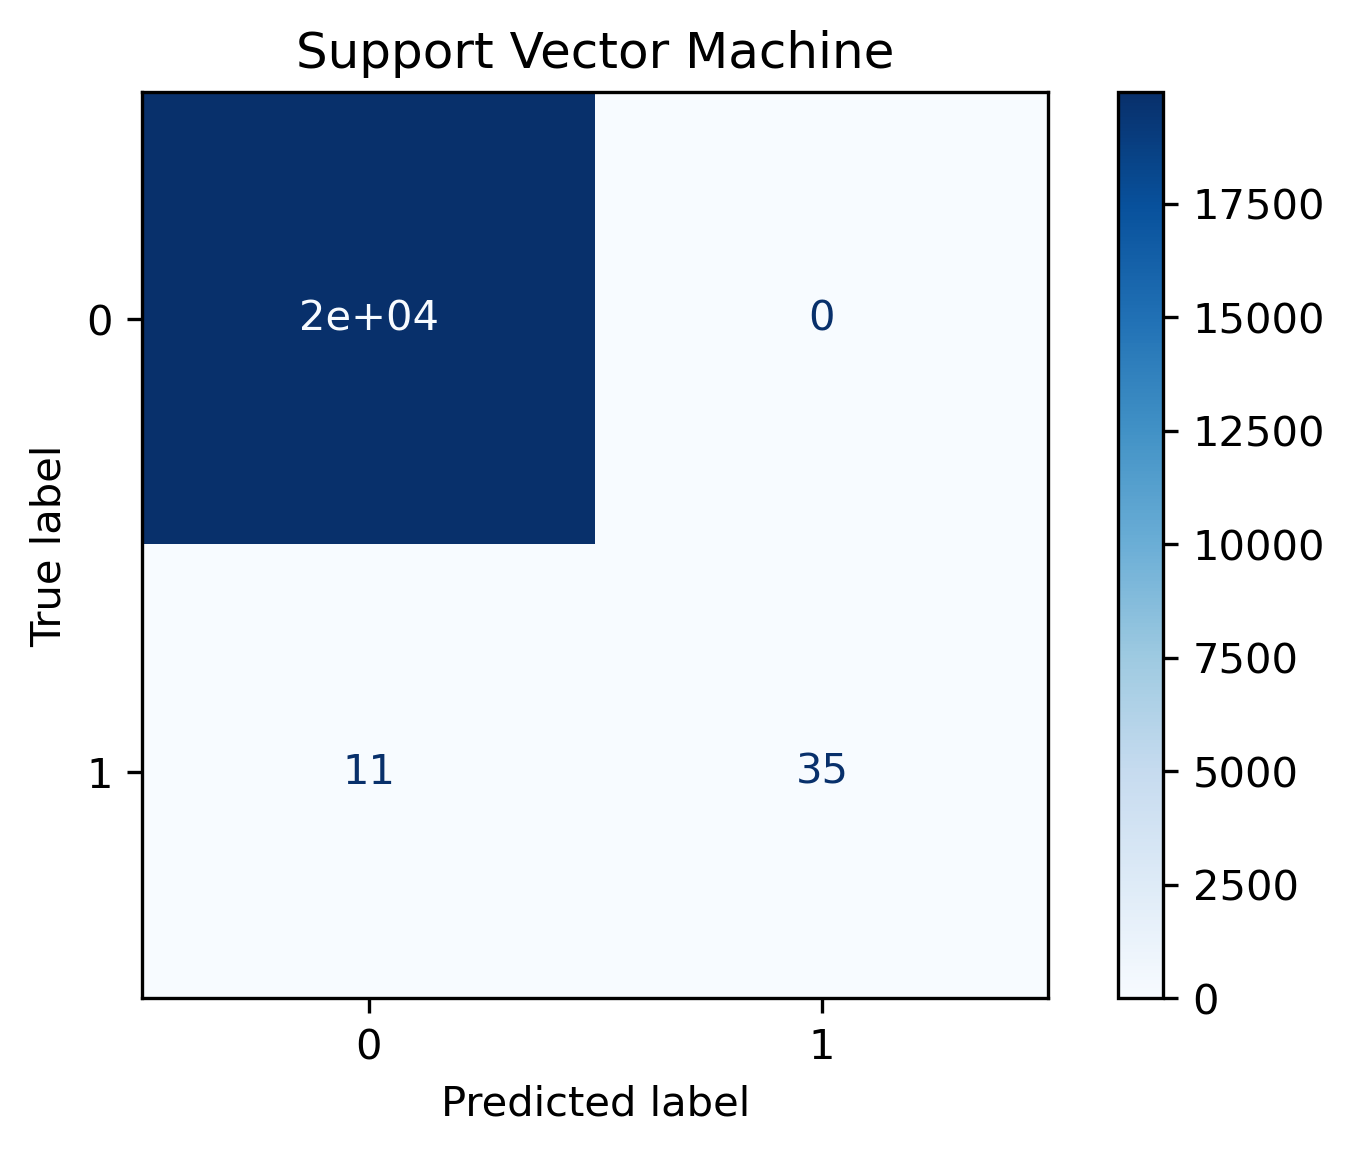
\includegraphics[width=\textwidth]{./images/svm_conf1.png}
    \label{fig:qqplotyyhatprice}
  \end{subfigure}
  \begin{subfigure}[b]{0.32\textwidth}
    \centering
    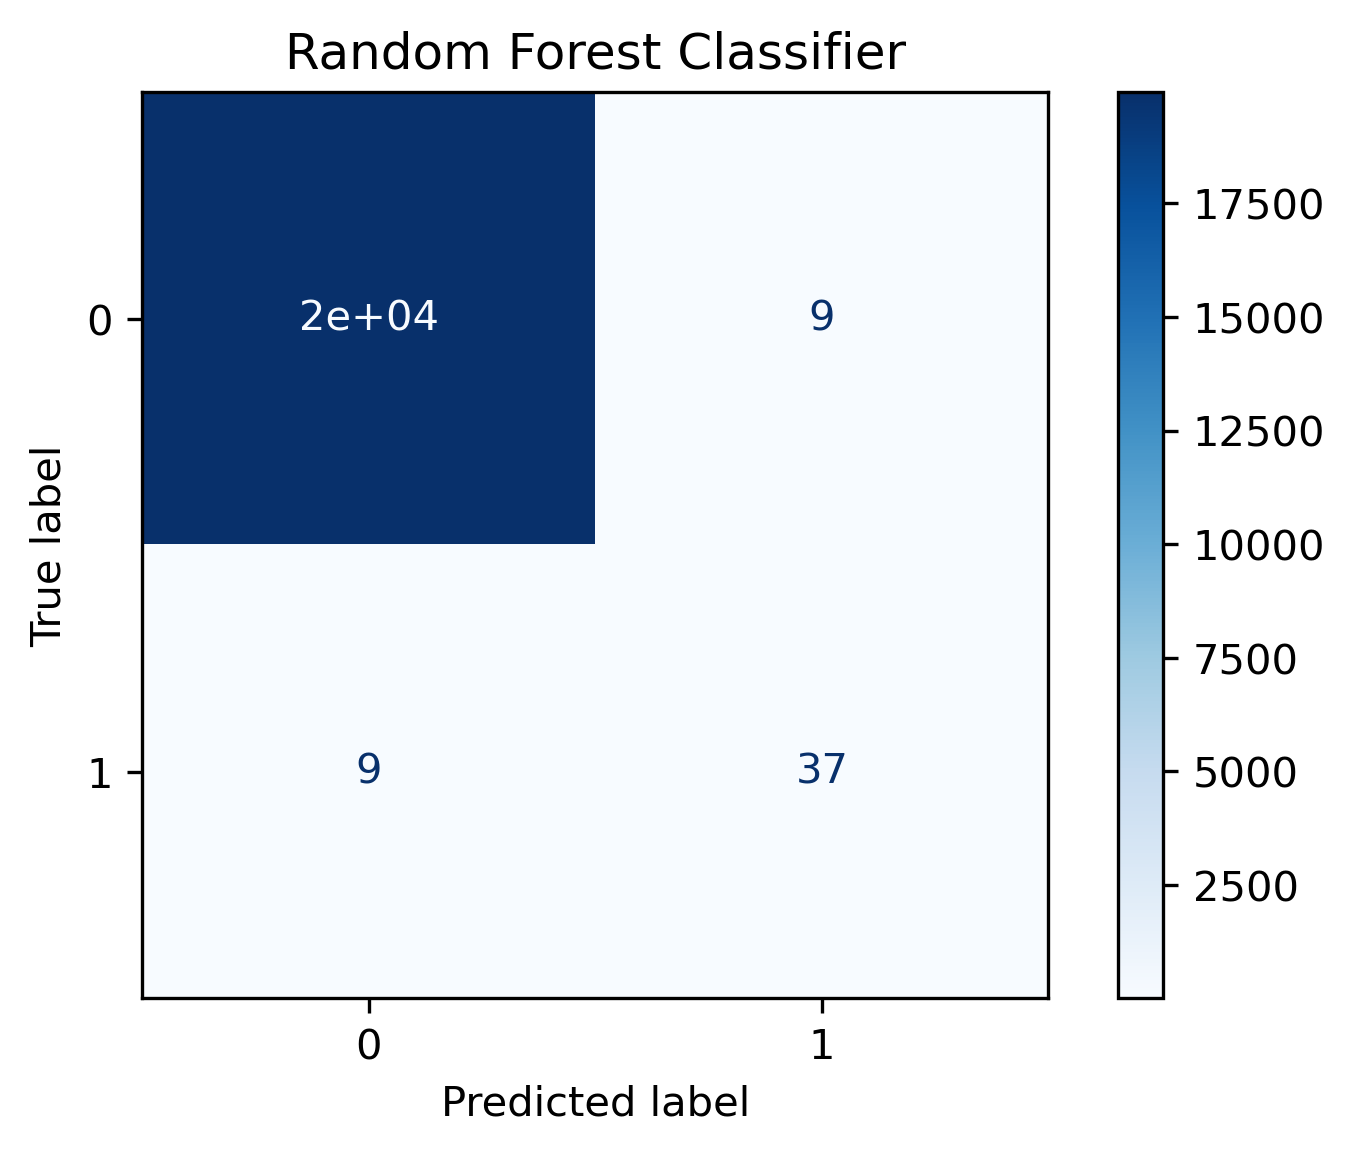
\includegraphics[width=\textwidth]{./images/rfc_conf1.png}
    \label{fig:scalelocationplotprice}
  \end{subfigure}
  \caption{Confusion matrices for logistic regression, SVM and Random Forest on test data}
  \label{fig:confusion1}
\end{figure}

\begin{table}[ht]
  \centering
  \caption{Accuracy, Precision, Recall and F1-Score for the 3 models}
  \label{tab:metrics1}
  \begin{tabular}{c|cccc}
    Model                    & Accuracy & Precision & Recall & F1-Score \\
    \hline
    Logistic Regression      & 0.9987   & 0.7027    & 0.6190 & 0.6582   \\
    Support Vector Machine   & 0.9994   & 0.9688    & 0.7381 & 0.8378   \\
    Random Forest Classifier & 0.9987   & 0.7027    & 0.6190 & 0.6582   \\
  \end{tabular}
\end{table}


\subsection{Constructing the Deep Neural Network}

Secondly we construct a deep neural network and compare it to the methods previously presented.
The network has an input layer with 30 nodes, one for each feature. Then there are $d$ fully connected hidden layers, each consisting of $k$ neurons. A ReLU layer is put in between each two neighboring hidden layers. In the end, there is one output node, to which a sigmoid function is applied, to convert scores to probabilities. If the output is greater or equal to 0.5 we classify a case as fraud, otherwise as non-fraud.
The model is trained using the ADAM Optimizer, reducing the binary cross entropy loss function. The training uses mini-batch gradient descent.
There are some parameters that we need to set in advance:
\begin{enumerate}
  \item The number of hidden layers $d$.
  \item The number of nodes in each hidden layer $k$.
  \item The learning rate $LR$.
  \item The $BATCH SIZE$, of batches used in the gradient descent.
  \item number of $EPOCHS$ (how many times to go over the entire dataset before stopping training)
\end{enumerate}
To perform a full grid search over all of these parameters would be very costly and take too much time, so we will try to figure out good parameters individually.

\subsubsection{Learning Rate}

For the learning rate the values $LR \in \{0.01, 0.001, 0.0001, 0.00001, 0.000001\}$ are considered while holding other values constant ($d=4,k=8, BATCH SIZE=64, EPOCHS=50$).
Table~\ref{tab:lrcomparison} shows the results for the resulting confusion matrices on the test data after 50 epochs of training. It seems like a learning rate of 0.0001 is best. The others mostly just classified the entire dataset as non-fraud.

\begin{table}[ht]
  \centering
  \caption{Performance for different Learning Rates on the test set}
  \label{tab:lrcomparison}

  \begin{tabular}{c|cccccccccc}
    LR       & TN    & TP & FP & FN & accuracy & F1     & loss (train) & loss (test) \\
    \hline
    0.01     & 19958 & 0  & 0  & 42 & 0.9979   & 0      & 0.2263       & 0.2100      \\
    0.001    & 19958 & 0  & 0  & 42 & 0.9979   & 0      & 0.2263       & 0.2060      \\
    0.0001   & 19946 & 25 & 12 & 17 & 0.9986   & 0.6329 & 0.0062       & 0.0051      \\
    0.00001  & 19946 & 0  & 0  & 42 & 0.9979   & 0      & 0.0121       & 0.0107      \\
    0.000001 & 19948 & 0  & 10 & 42 & 0.9974   & 0      & 0.5478       & 0.5474      \\
  \end{tabular}

\end{table}

Next we will take a look at the influence of the size and amount of hidden layers: In the following Table~\ref{tab:sizecomparison} you can see the training outcomes for different configurations, keeping other values constant ($BATCH SIZE=64, EPOCHS=50, LR=0.0001$). The configurations $(d,k)$ = (hidden layer count, nodes per hidden layer) are set to $(1,8)$, $(1,16)$, $(4,8)$, $(4,16)$ and $(8,8)$. Surprisingly having 4 hidden layers with 8 nodes each seems to be the best configuration.


\begin{table}[ht]
  \centering
  \caption{Performance for different Learning Rates on the test set}
  \label{tab:sizecomparison}
  \begin{tabular}{cc|cccccccc}
    d & k  & TN    & TP & FP & FN & accuracy & F1     & loss (train) & loss (test) \\
    \hline
    1 & 8  & 19958 & 0  & 0  & 42 & 0.9979   & 0      & 0.2252       & 0.2057      \\
    1 & 16 & 19954 & 0  & 0  & 46 & 0.9979   & 0      & 0.2216       & 0.2300      \\
    4 & 8  & 19946 & 25 & 12 & 17 & 0.9986   & 0.6329 & 0.0062       & 0.0051      \\
    4 & 16 & 19947 & 20 & 11 & 22 & 0.99835  & 0.5479 & 0.008        & 0.0065      \\
    8 & 8  & 19950 & 9  & 8  & 33 & 0.9974   & 0.3051 & 0.0115       & 0.0103      \\
  \end{tabular}
\end{table}

For the rest of this report we will consider a network with the following parameters:
\begin{enumerate}
  \item The number of hidden layer $d = 4$.
  \item The number of nodes in each hidden layer $k = 8$.
  \item $LR = 0.0001$.
  \item $BATCH SIZE = 64$
  \item $EPOCHS = 50$
\end{enumerate}

\subsection{Characteristics of the DNN}

Table~\ref{tab:chars} shows some characteristics of the deep neural network that was deemed best during the hyper parameter selection process:

\begin{table}[ht]
  \centering
  \caption{Performance of the strongest model}
  \label{tab:chars}
  \begin{tabular}{c|cc}
    characteristic & train  & test   \\
    \hline
    TN             & 79790  & 19946  \\
    TP             & 114    & 25     \\
    FP             & 28     & 12     \\
    FN             & 67     & 17     \\
    Accuracy       & 0.9988 & 0.9986 \\
    Precision      & 0.8028 & 0.6757 \\
    Recall         & 0.6298 & 0.5952 \\
    F1             & 0.7058 & 0.6329 \\
    Loss           & 0.0062 & 0.0051 \\
  \end{tabular}
\end{table}

Figure~\ref{fig:accuracy_and_loss} shows how accuracy and loss devoloped throughout the training period for both the train and test dataset. Figure~\ref{fig:confusion_matrices} shows the confusion matrices on the train and test datasets after the model was trained for 50 epochs.

\begin{figure}[htb]
  \centering
  \begin{subfigure}[b]{0.48\textwidth}
    \centering
    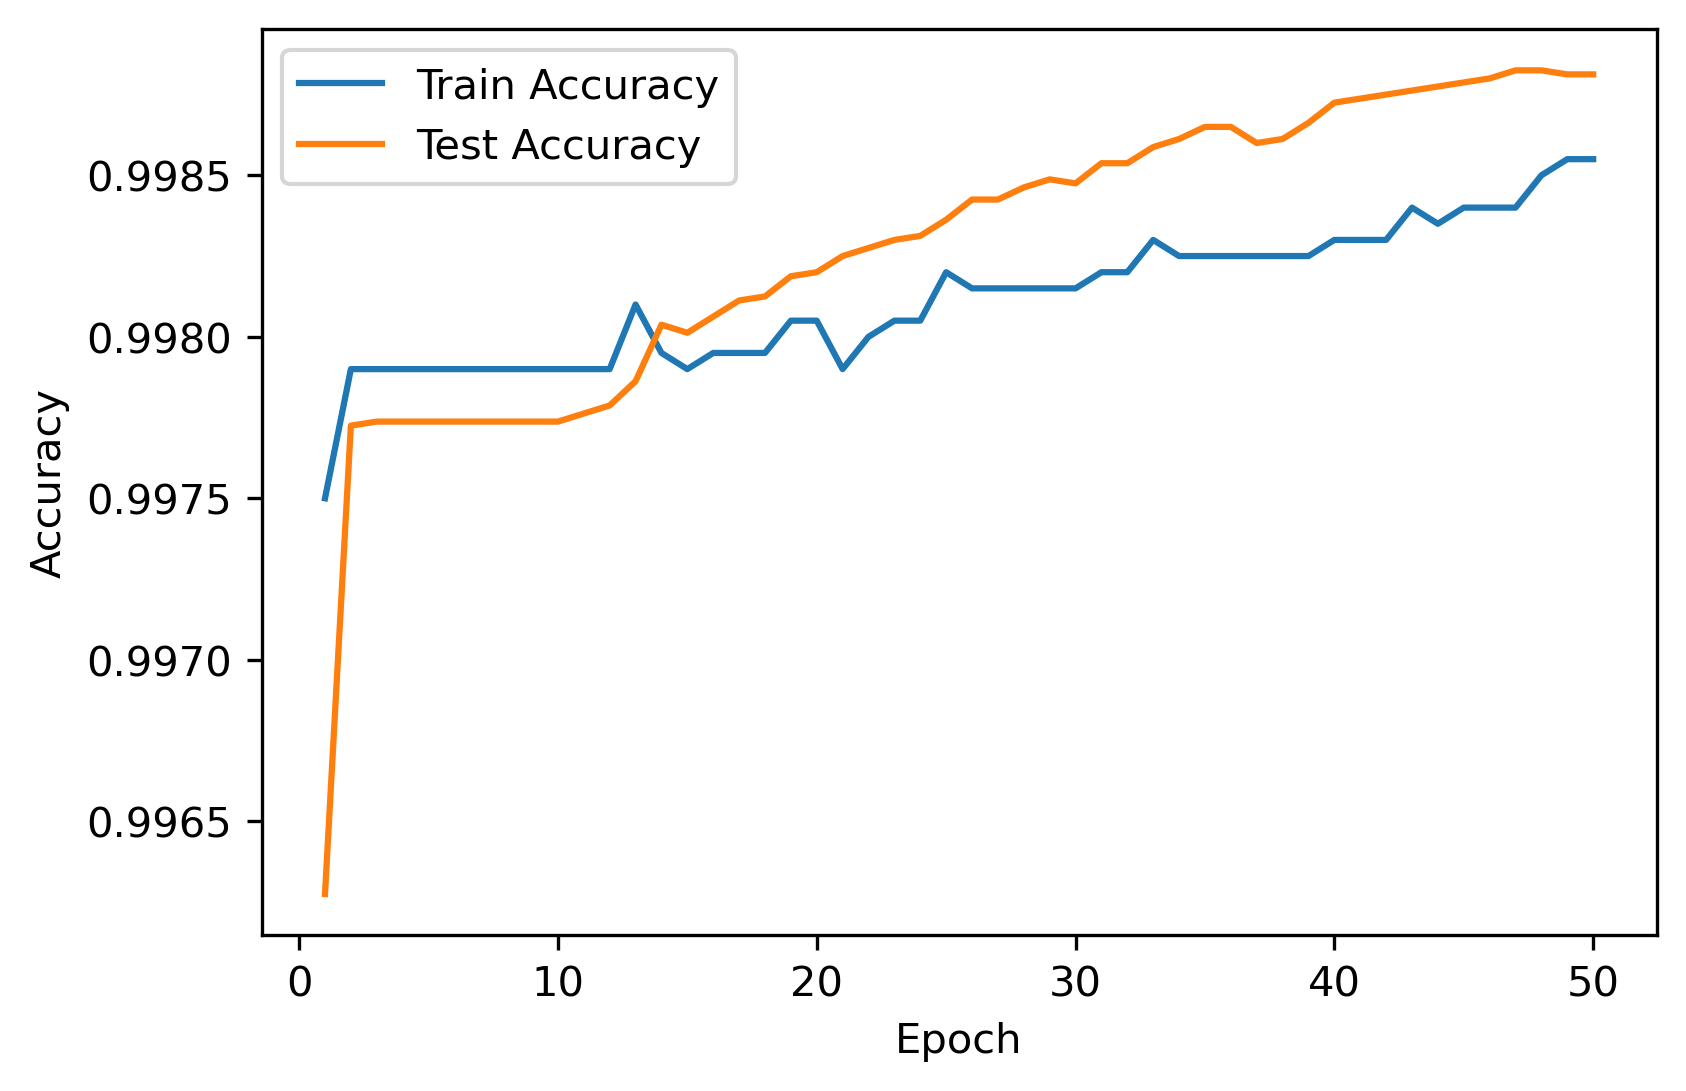
\includegraphics[width=\textwidth]{./images/net(d4_k8)_E50_LR0.0001_B64/accuracy.png}
    \label{fig:accuracy}
  \end{subfigure}
  \begin{subfigure}[b]{0.48\textwidth}
    \centering
    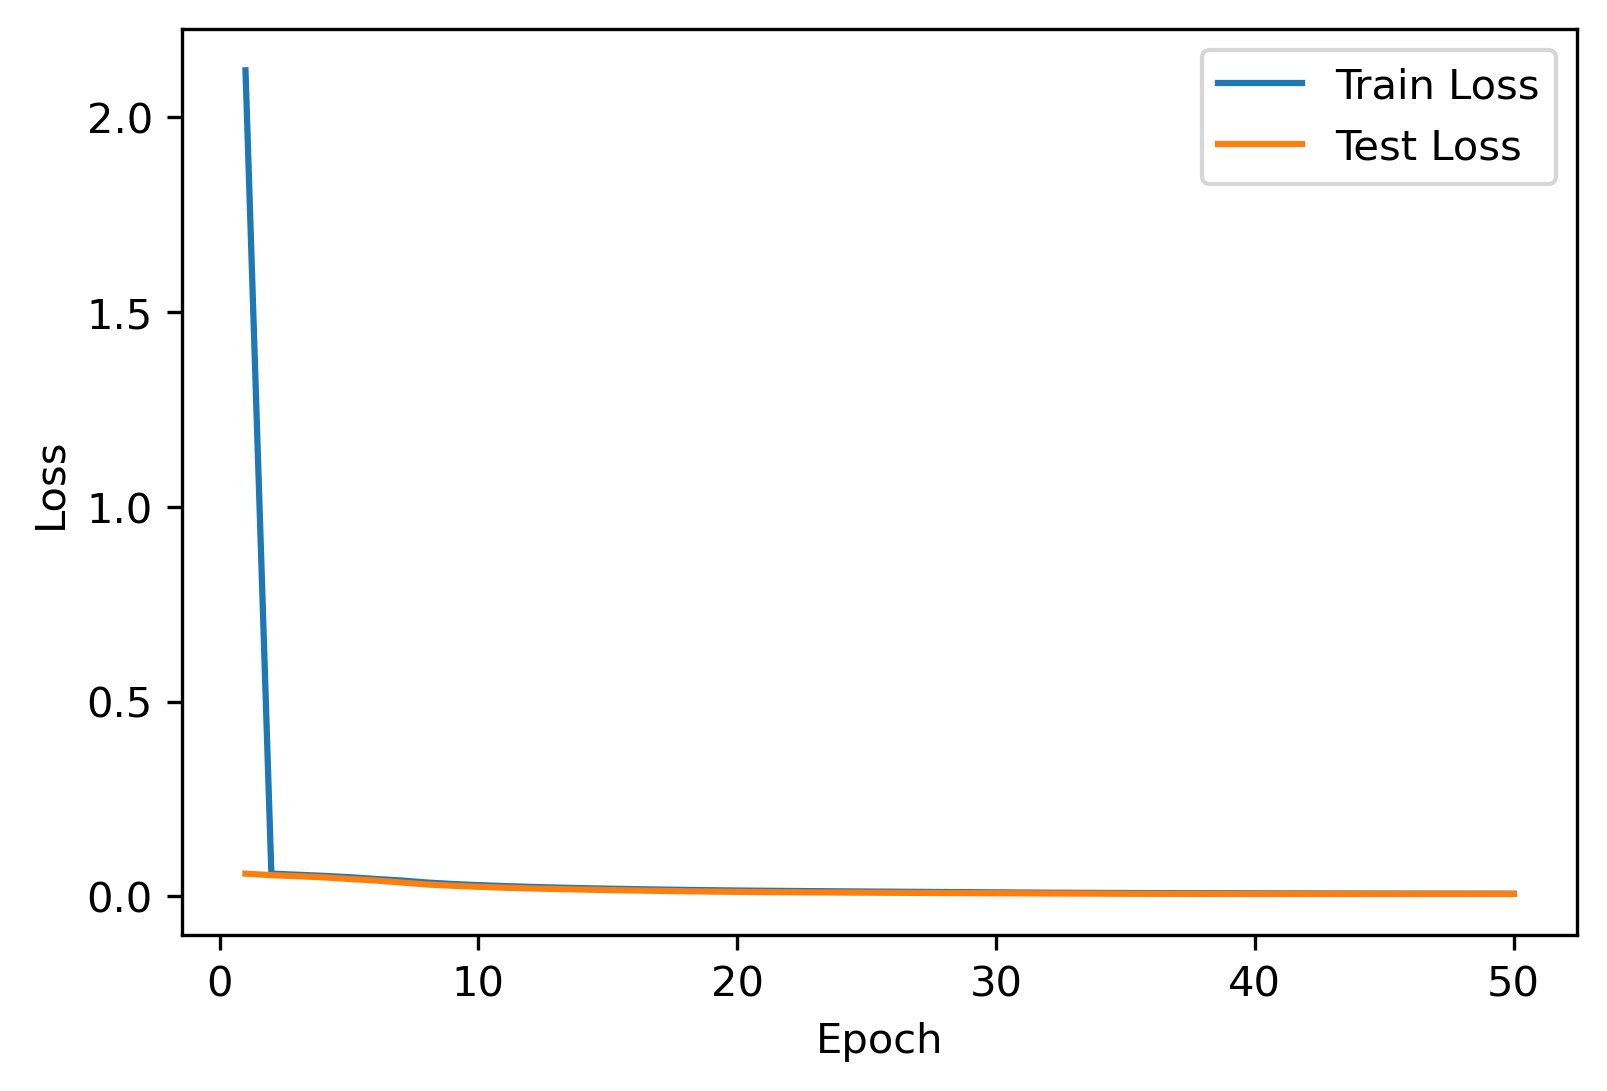
\includegraphics[width=\textwidth]{./images/net(d4_k8)_E50_LR0.0001_B64/loss.png}
    \label{fig:loss}
  \end{subfigure}
  \caption{Accuracy and Loss over the training period}
  \label{fig:accuracy_and_loss}
\end{figure}


\begin{figure}[htb]
  \centering
  \begin{subfigure}[b]{0.48\textwidth}
    \centering
    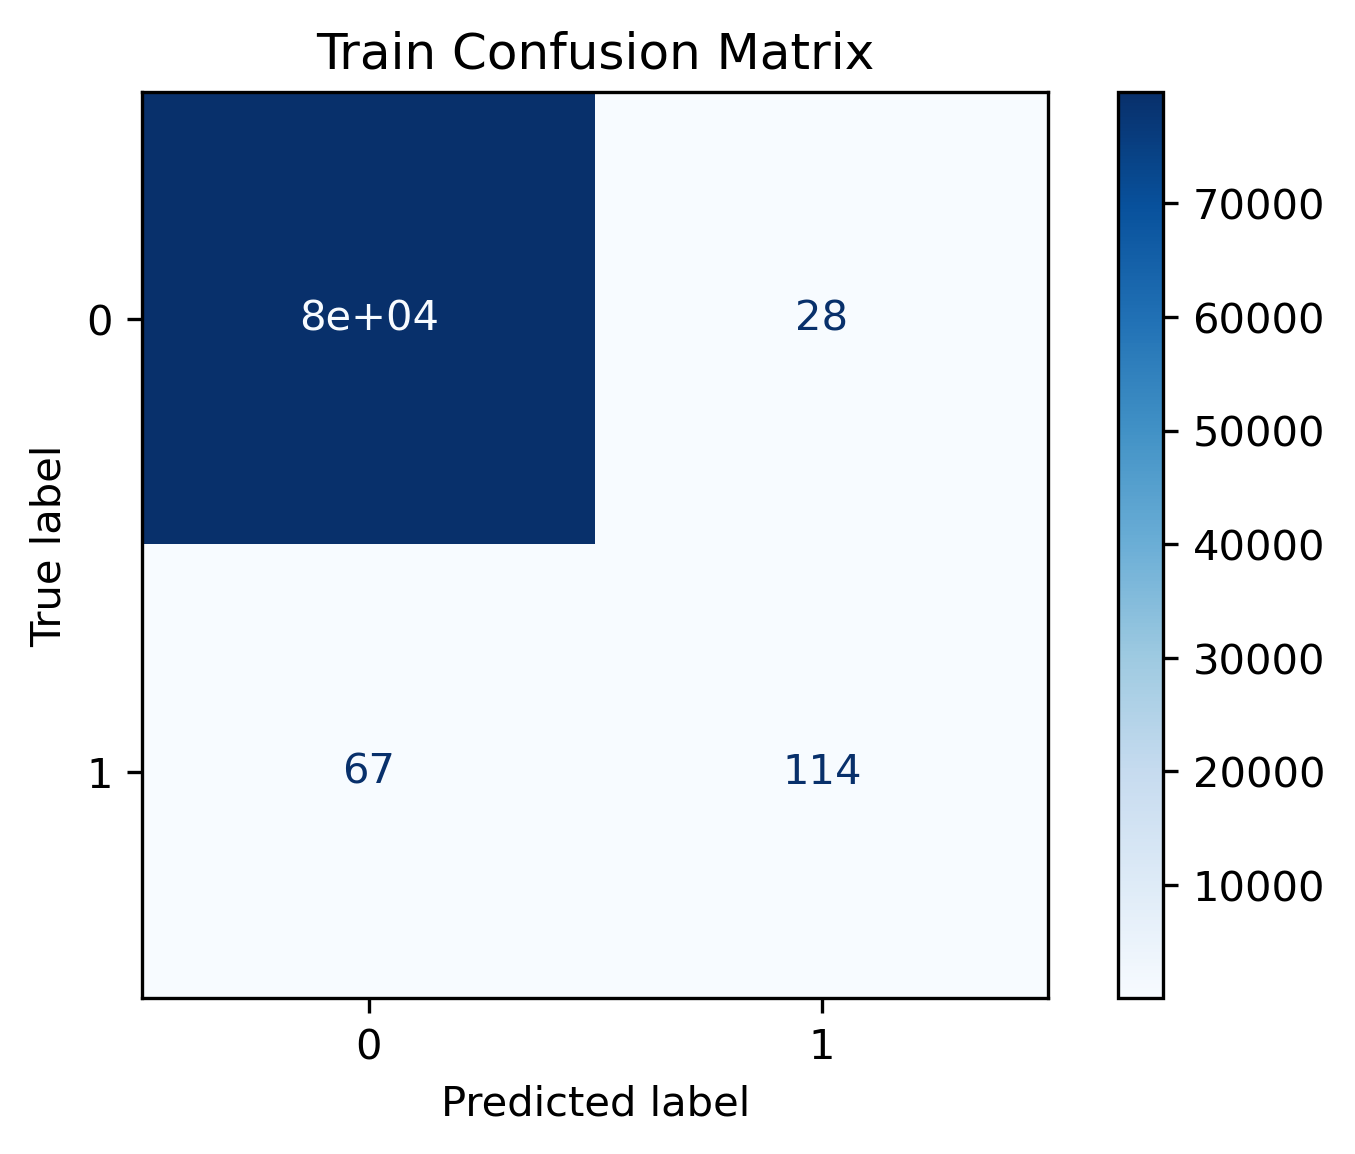
\includegraphics[width=\textwidth]{./images/net(d4_k8)_E50_LR0.0001_B64/conf_train.png}
    \label{fig:confusion_train}
  \end{subfigure}
  \begin{subfigure}[b]{0.48\textwidth}
    \centering
    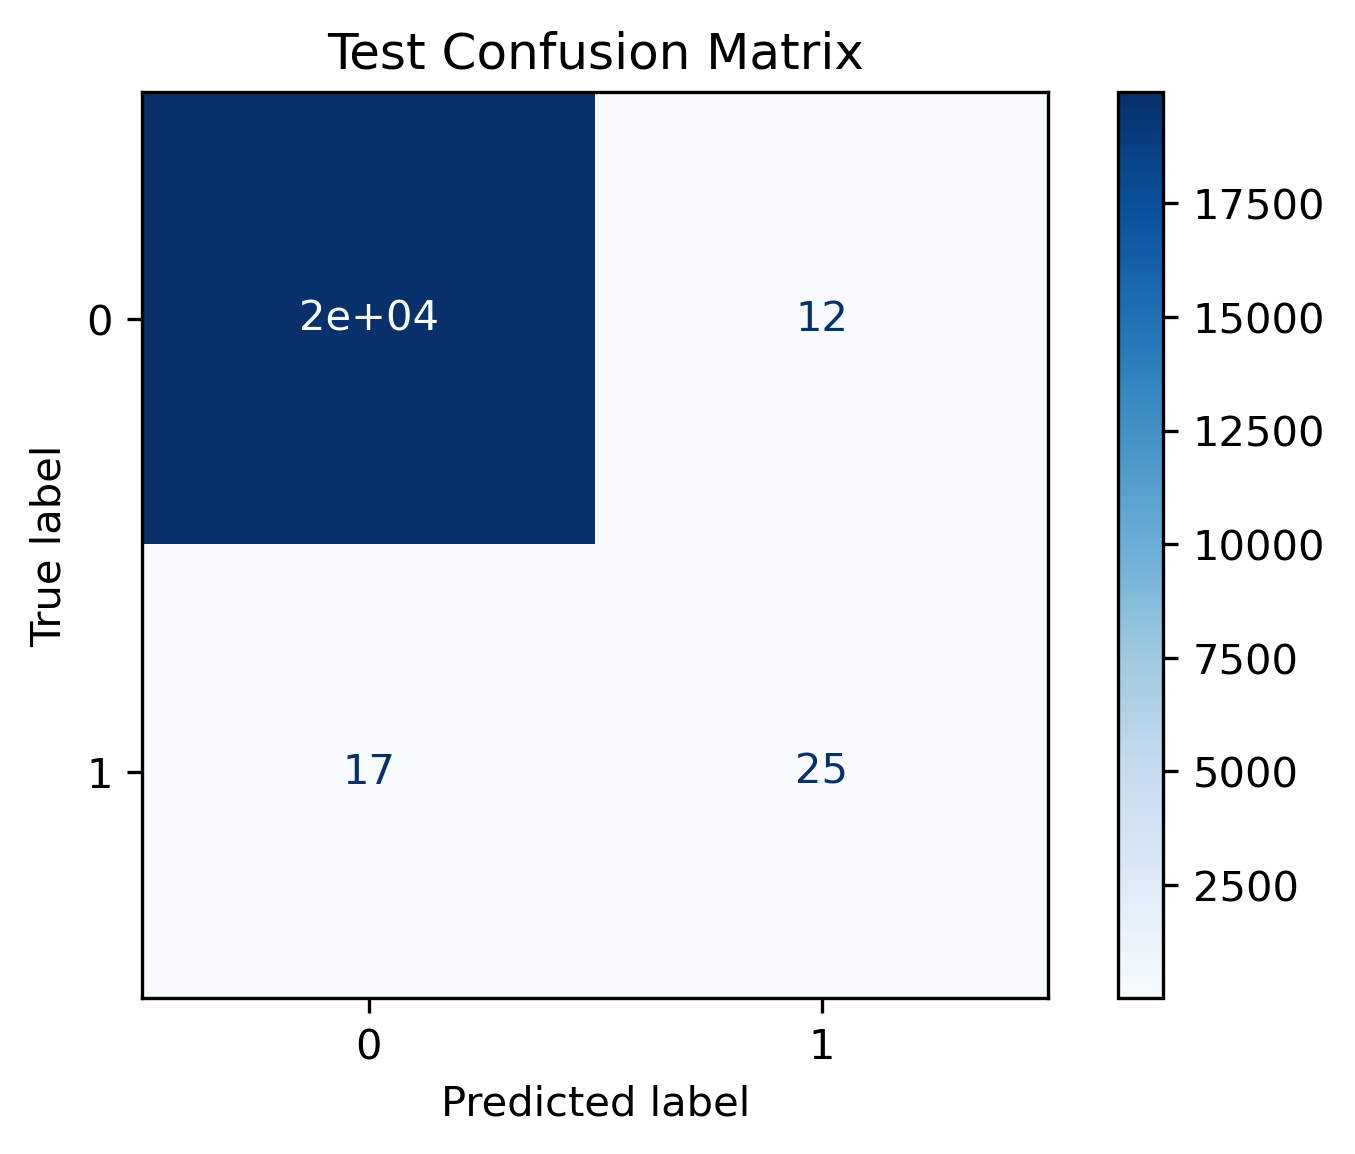
\includegraphics[width=\textwidth]{./images/net(d4_k8)_E50_LR0.0001_B64/conf_test.png}
    \label{fig:confusion_test}
  \end{subfigure}
  \caption{Confusion matrices for test and train data}
  \label{fig:confusion_matrices}
\end{figure}

\subsection{ROC and PRC curves}

Figure~\ref{fig:roc_and_prc} shows the ROC and PRC curves of the 4 different models and also provides the area under curve for each.

\begin{figure}[htb]
  \centering
  \begin{subfigure}[b]{0.48\textwidth}
    \centering
    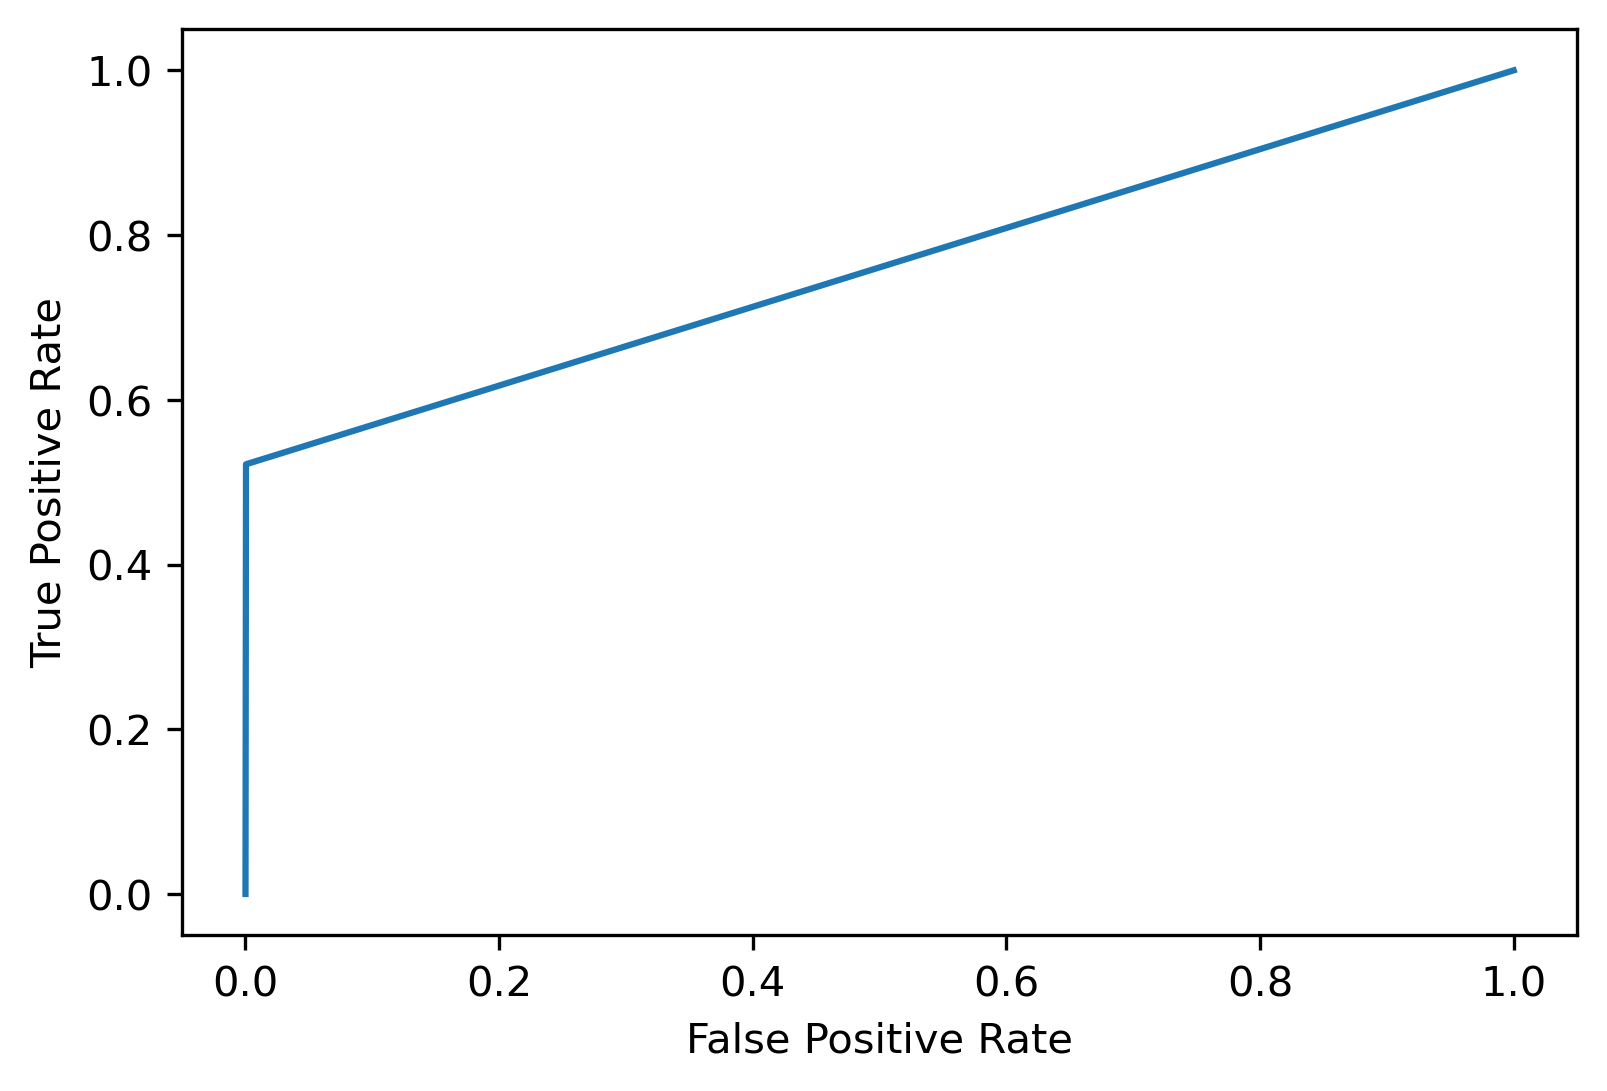
\includegraphics[width=\textwidth]{./images/net(d4_k8)_E50_LR0.0001_B64/roc.png}
    \caption{ROC for DNN. AUC = 0.7973}
    \label{fig:dnn_roc}
  \end{subfigure}
  \begin{subfigure}[b]{0.48\textwidth}
    \centering
    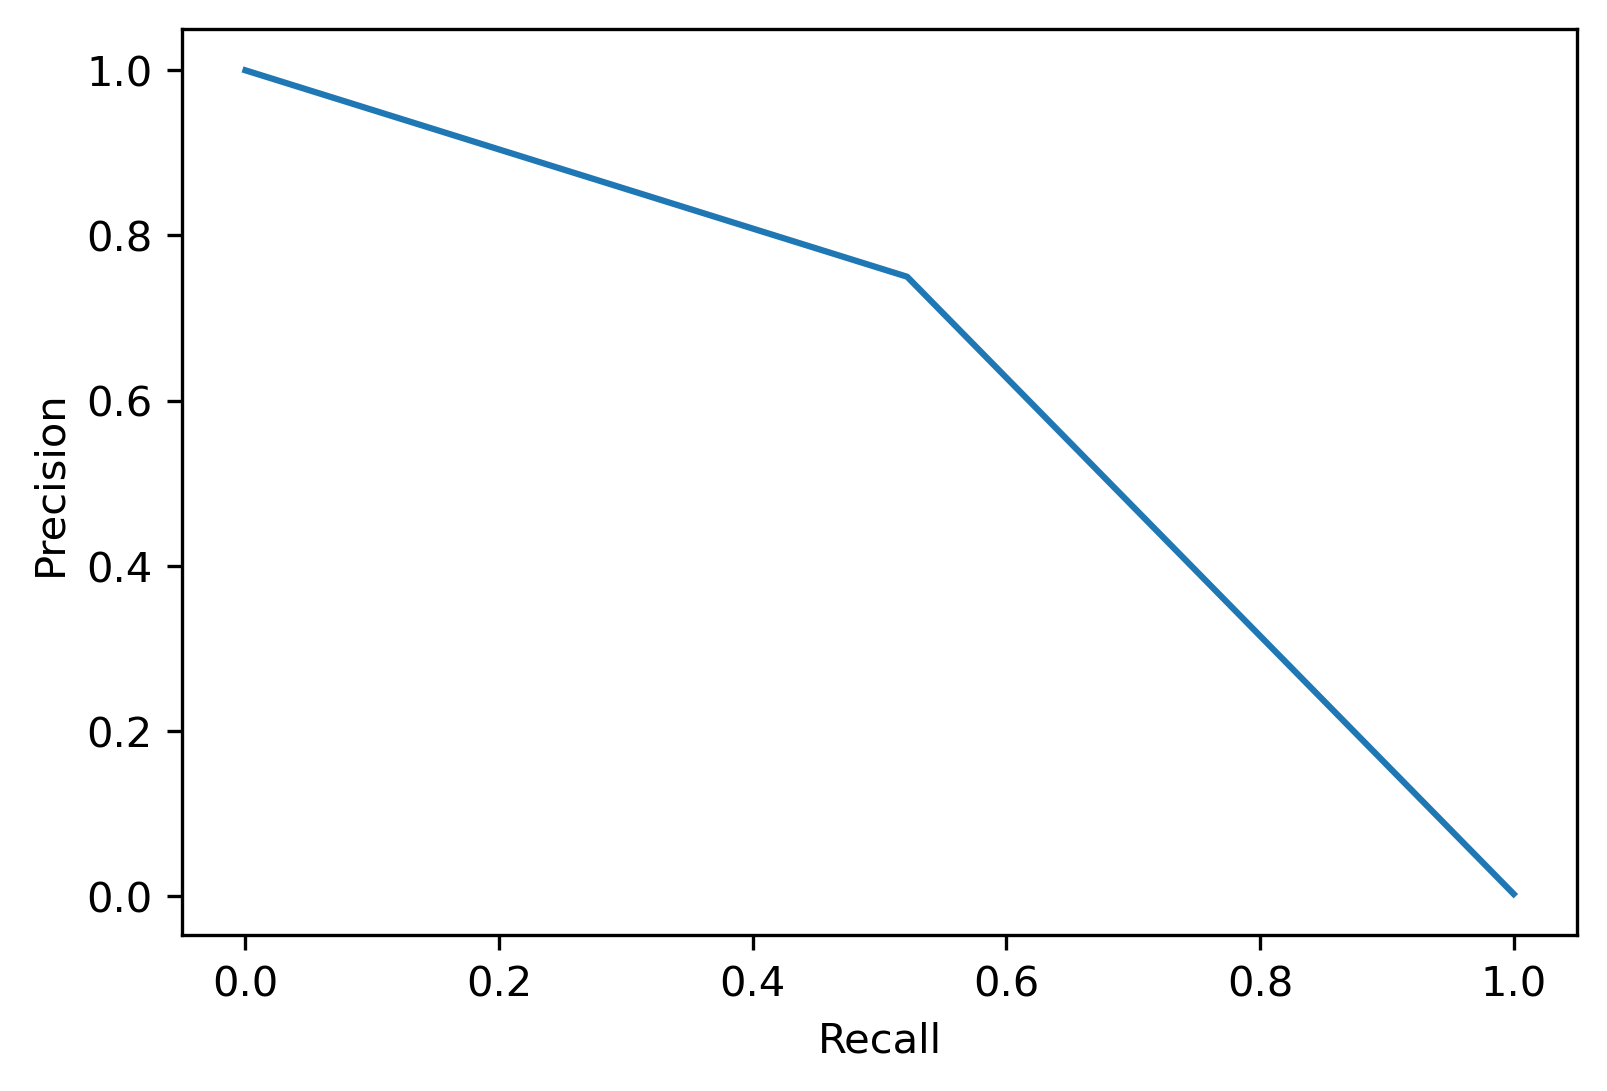
\includegraphics[width=\textwidth]{./images/net(d4_k8)_E50_LR0.0001_B64/prc.png}
    \caption{ROC for DNN. AUC = 0.4030}
    \label{fig:dnn_orc}
  \end{subfigure}
  \begin{subfigure}[b]{0.48\textwidth}
    \centering
    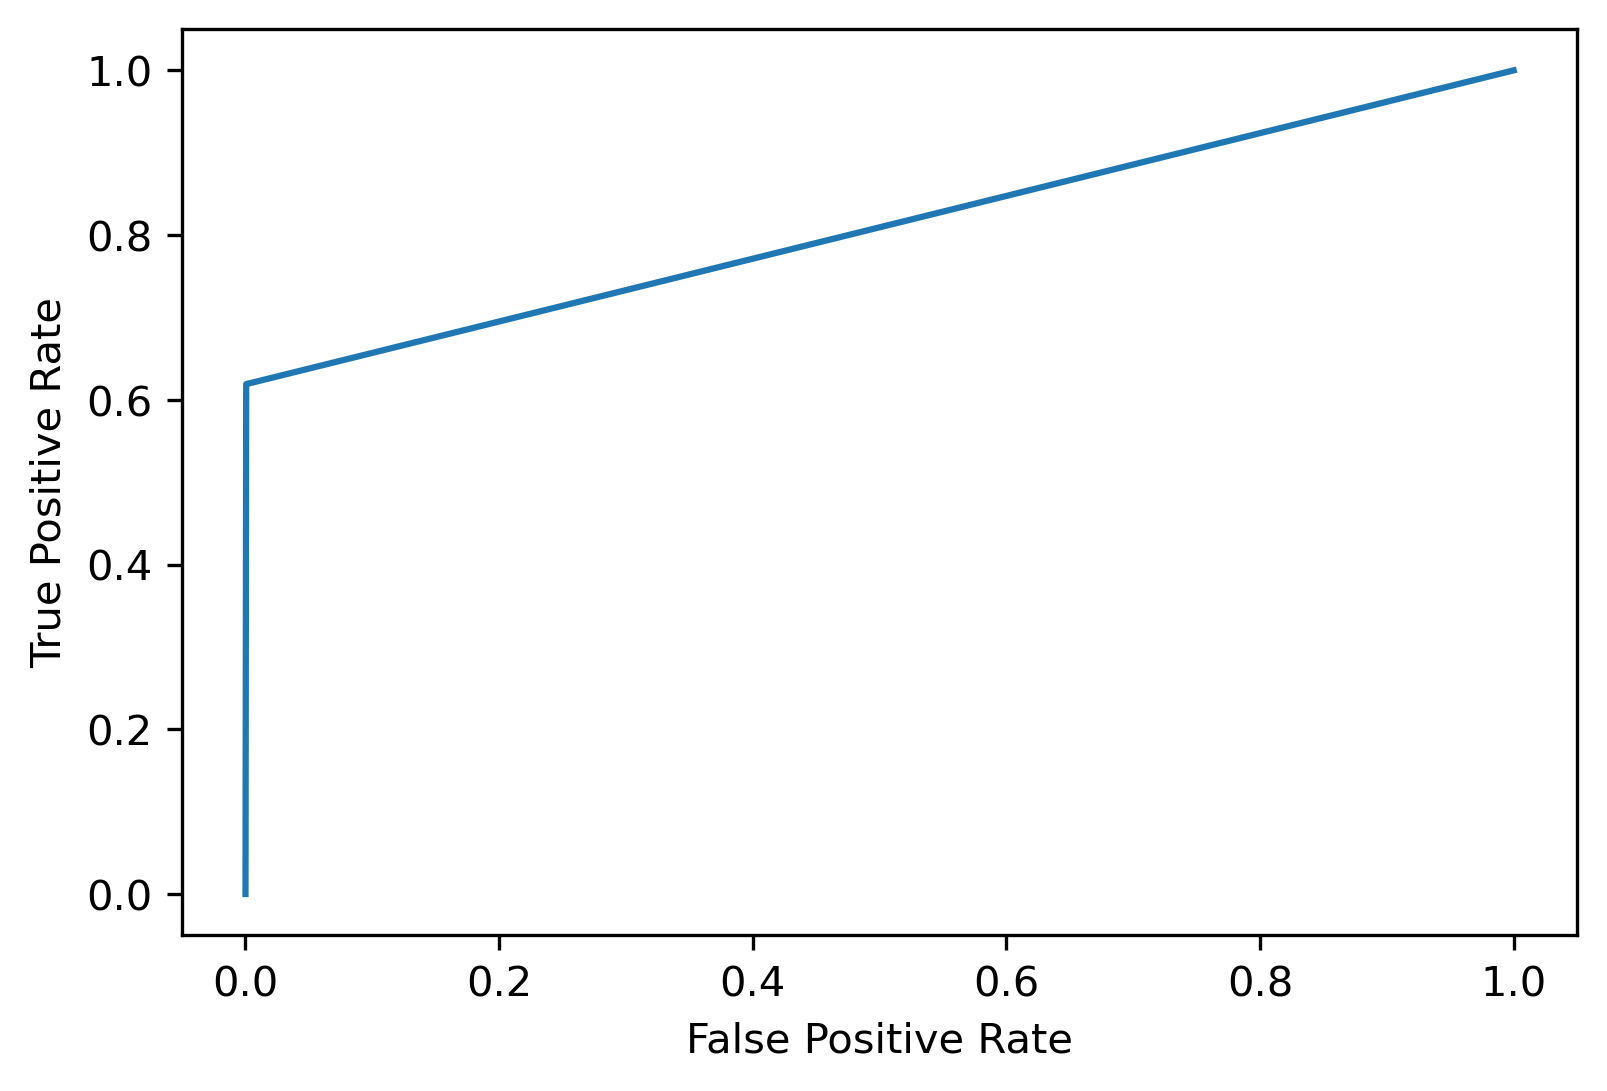
\includegraphics[width=\textwidth]{./images/reg_roc.png}
    \caption{ROC for Logistic Regression. AUC = 0.8092}
    \label{fig:reg_roc}
  \end{subfigure}
  \begin{subfigure}[b]{0.48\textwidth}
    \centering
    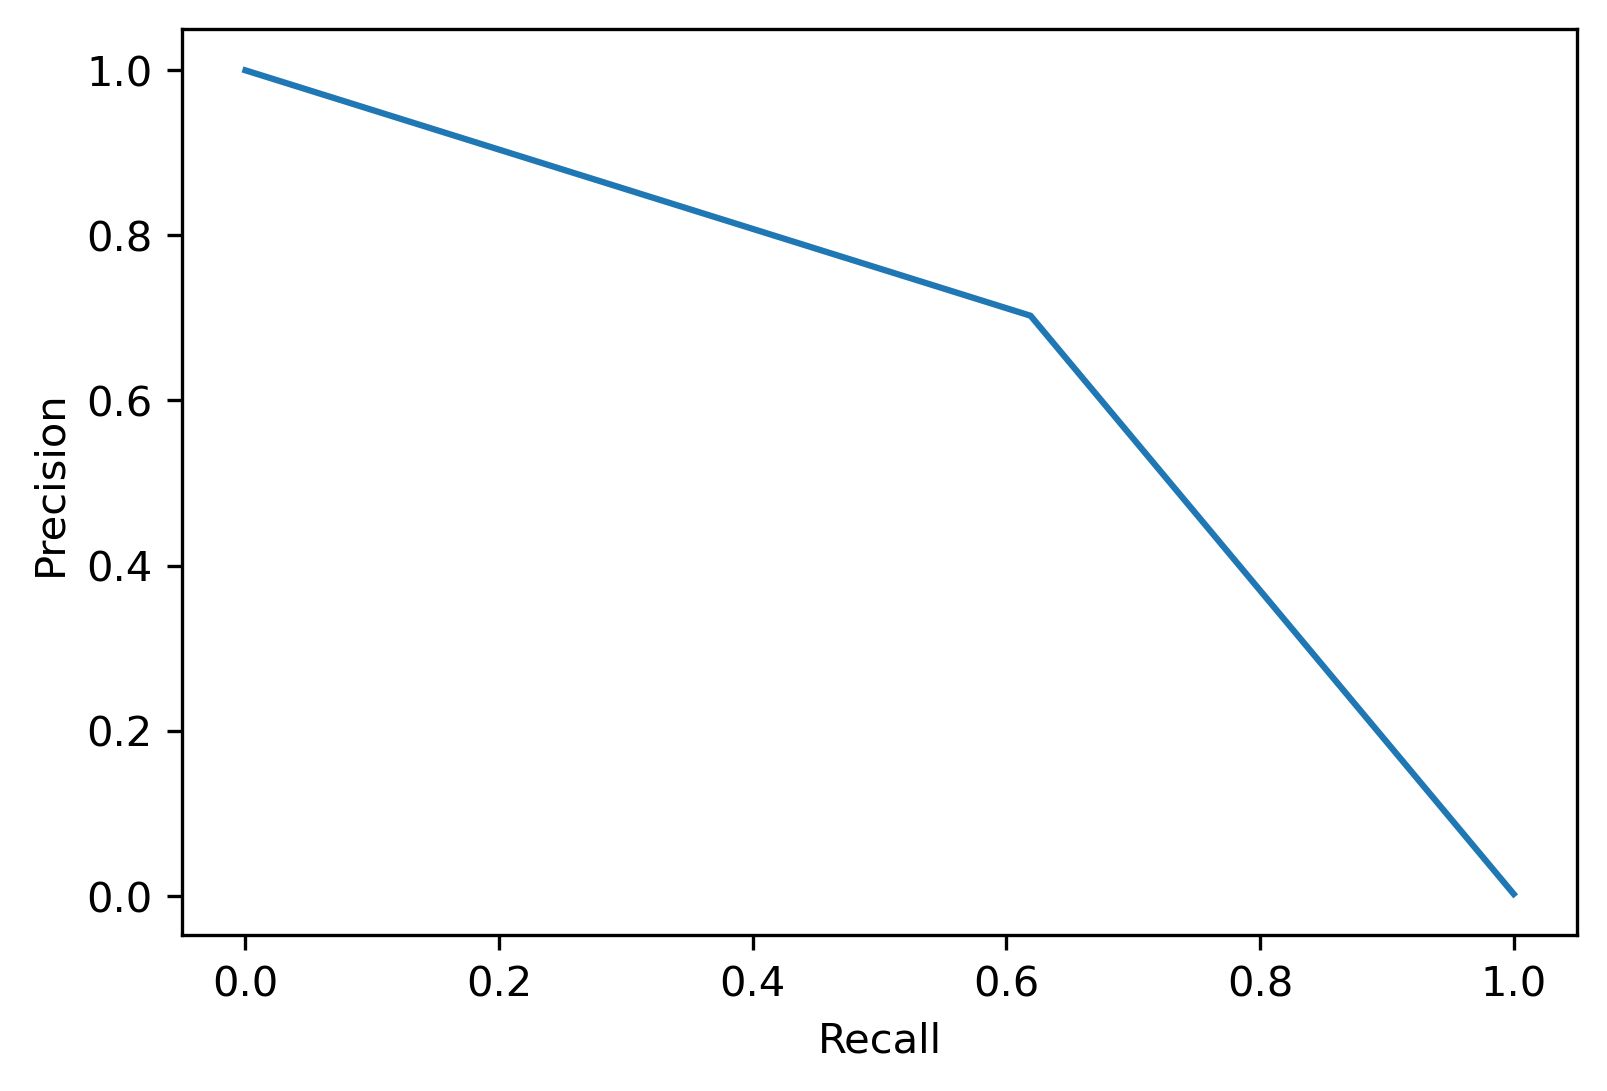
\includegraphics[width=\textwidth]{./images/reg_prc.png}
    \caption{PRC for Logistic Regression. AUC = 0.4358}
    \label{fig:reg_prc}
  \end{subfigure}
  \begin{subfigure}[b]{0.48\textwidth}
    \centering
    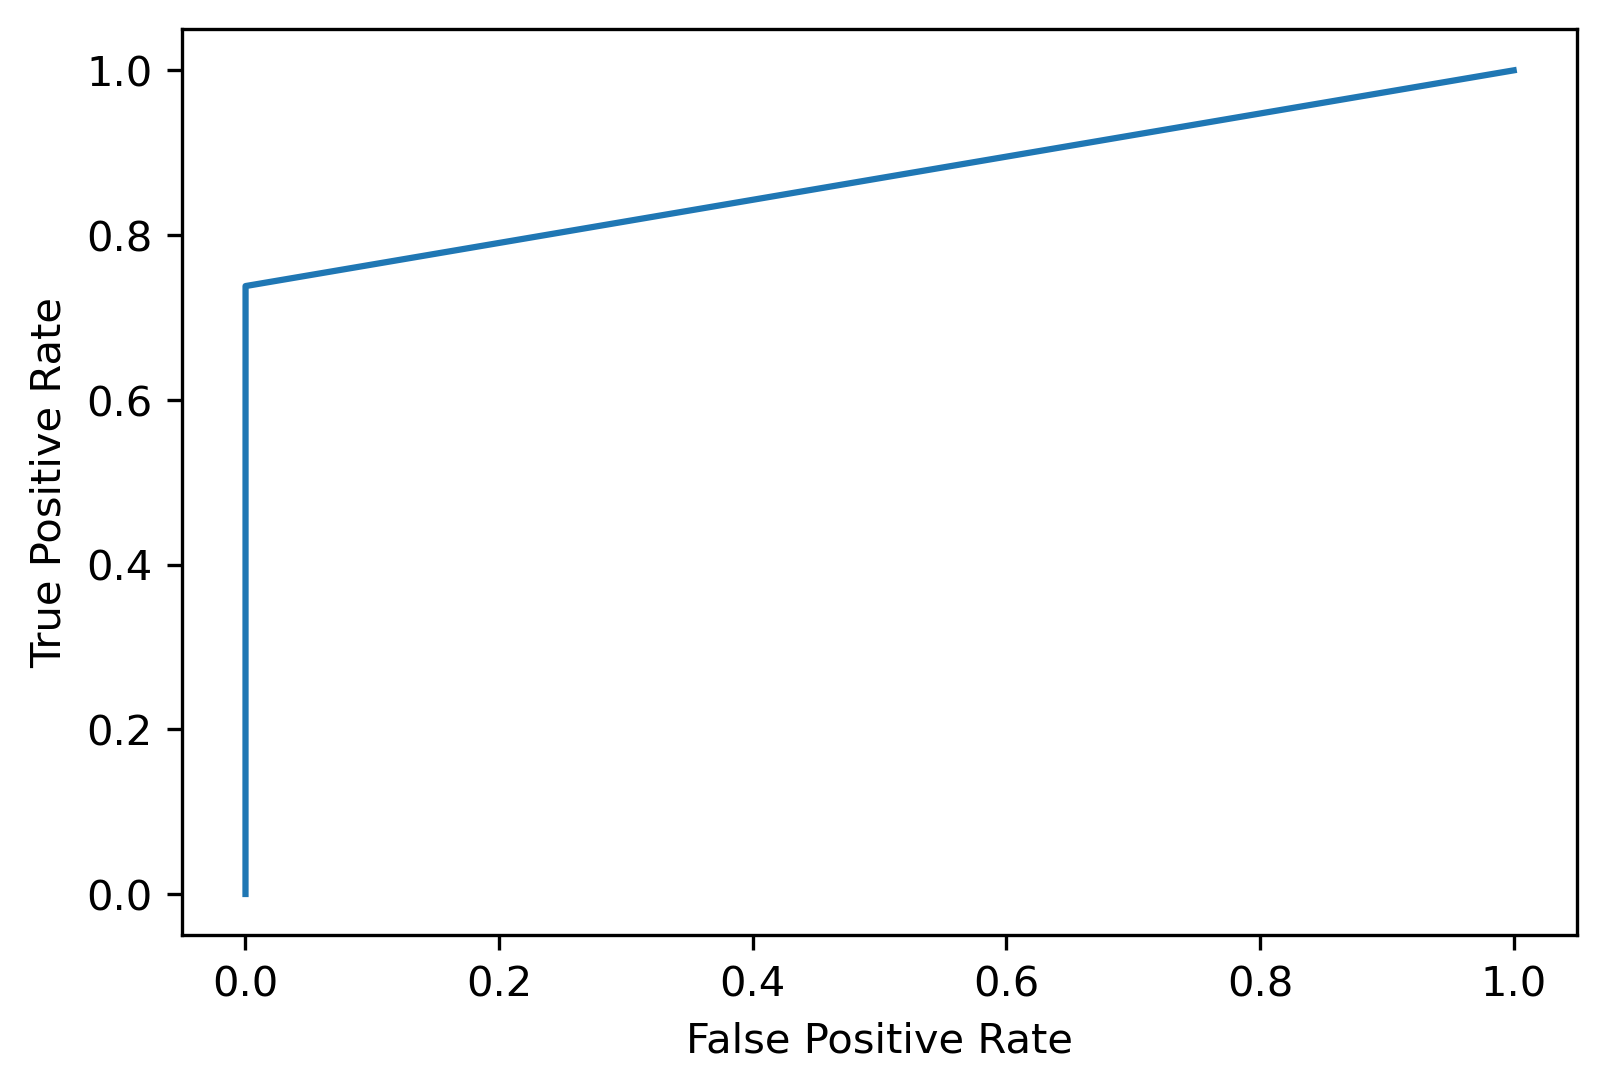
\includegraphics[width=\textwidth]{./images/svm_roc.png}
    \caption{ROC for Support Vector Machine. AUC = 0.869}
    \label{fig:svm_roc}
  \end{subfigure}
  \begin{subfigure}[b]{0.48\textwidth}
    \centering
    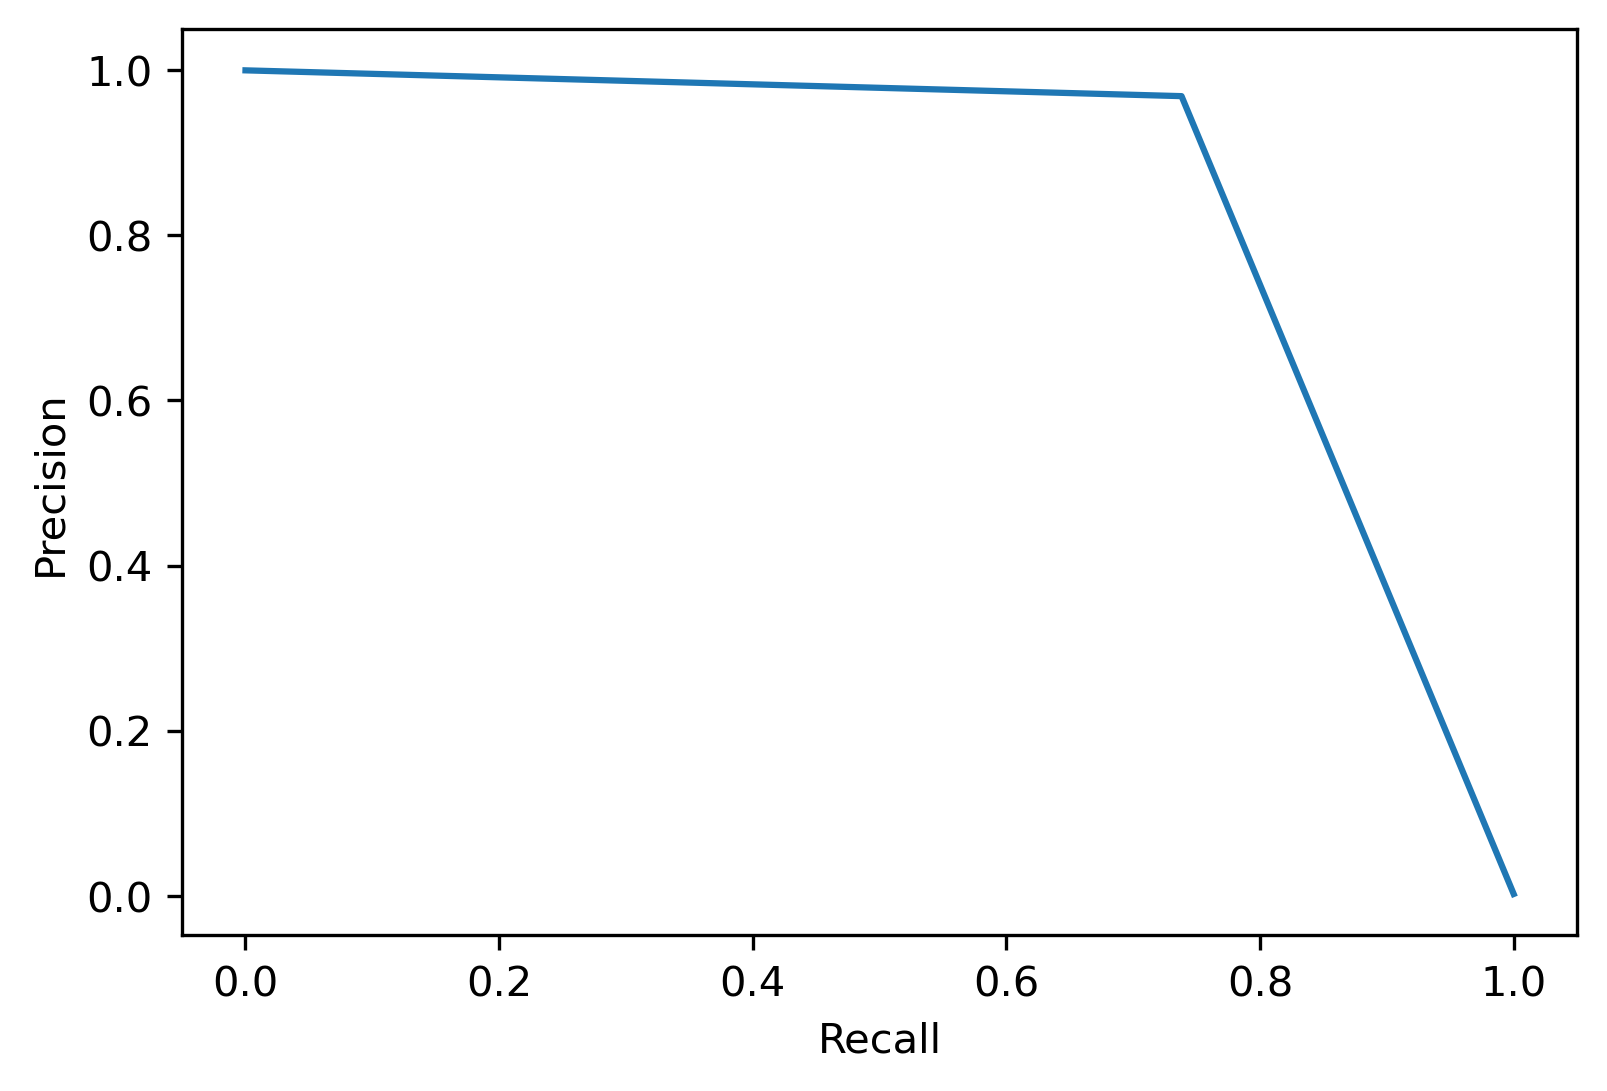
\includegraphics[width=\textwidth]{./images/svm_prc.png}
    \caption{PRC for Support Vector Machine. AUC = 0.7156}
    \label{fig:svm_prc}
  \end{subfigure}
  \begin{subfigure}[b]{0.48\textwidth}
    \centering
    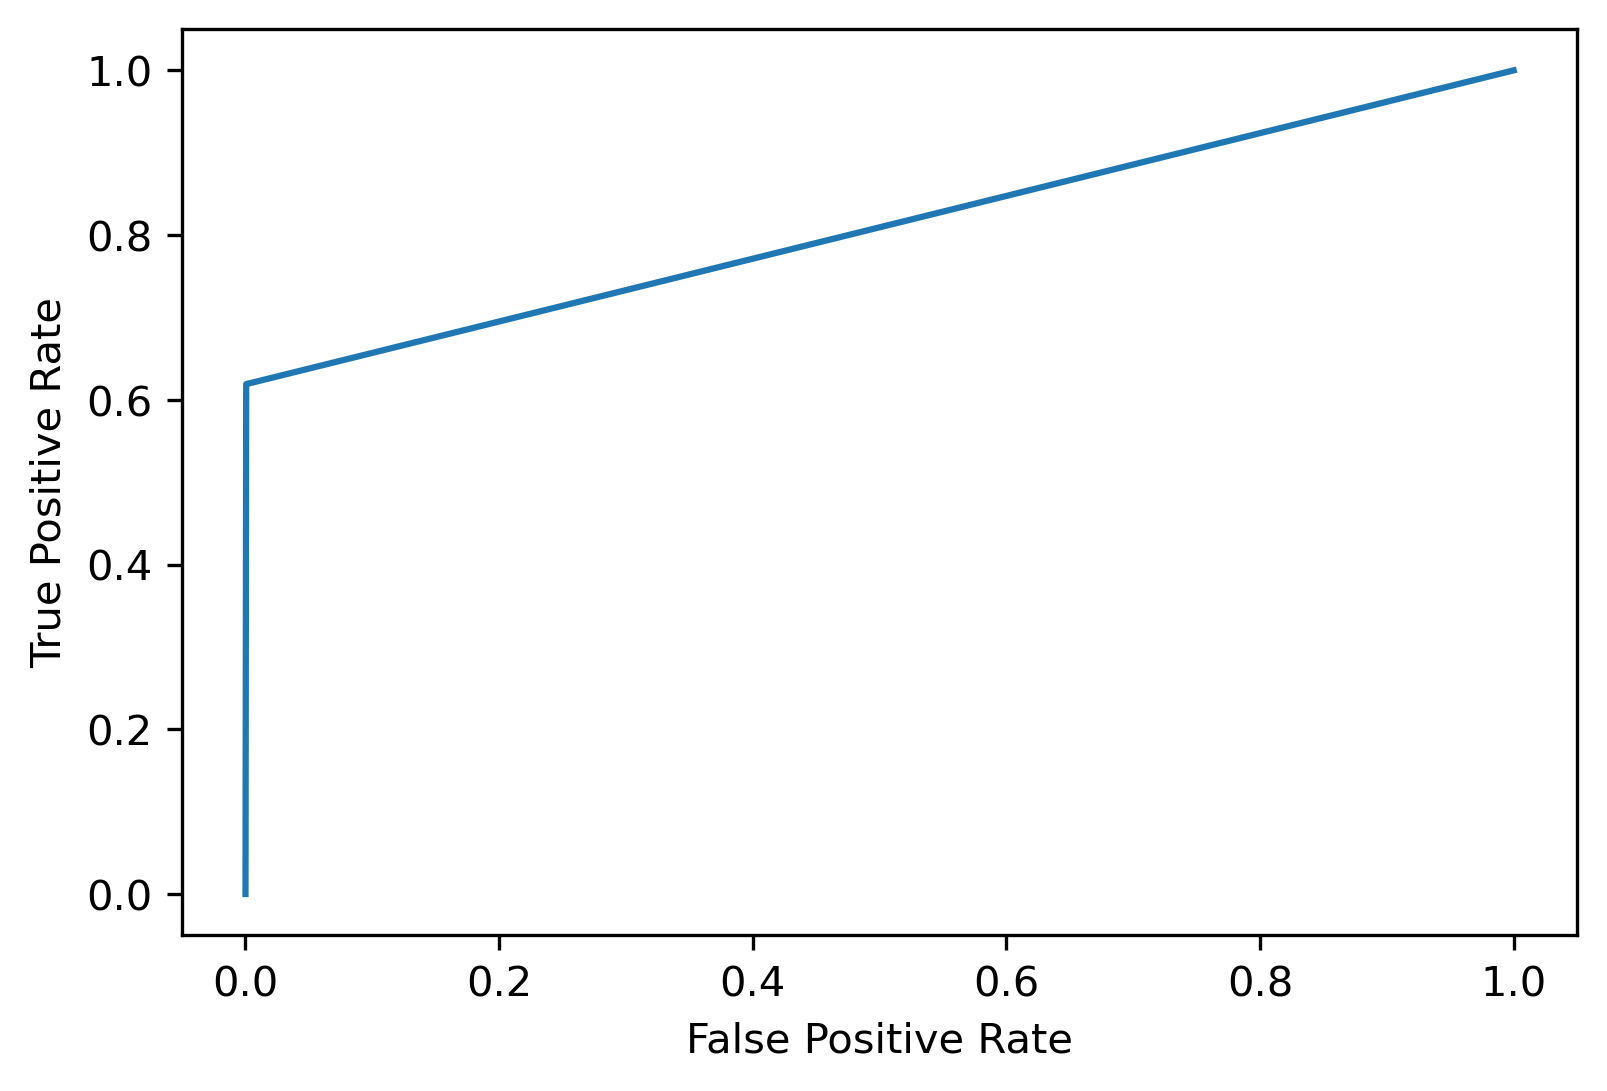
\includegraphics[width=\textwidth]{./images/rfc_roc.png}
    \caption{ROC for Random Forest Classifier. AUC = 0.8092}
    \label{fig:rfc_roc}
  \end{subfigure}
  \begin{subfigure}[b]{0.48\textwidth}
    \centering
    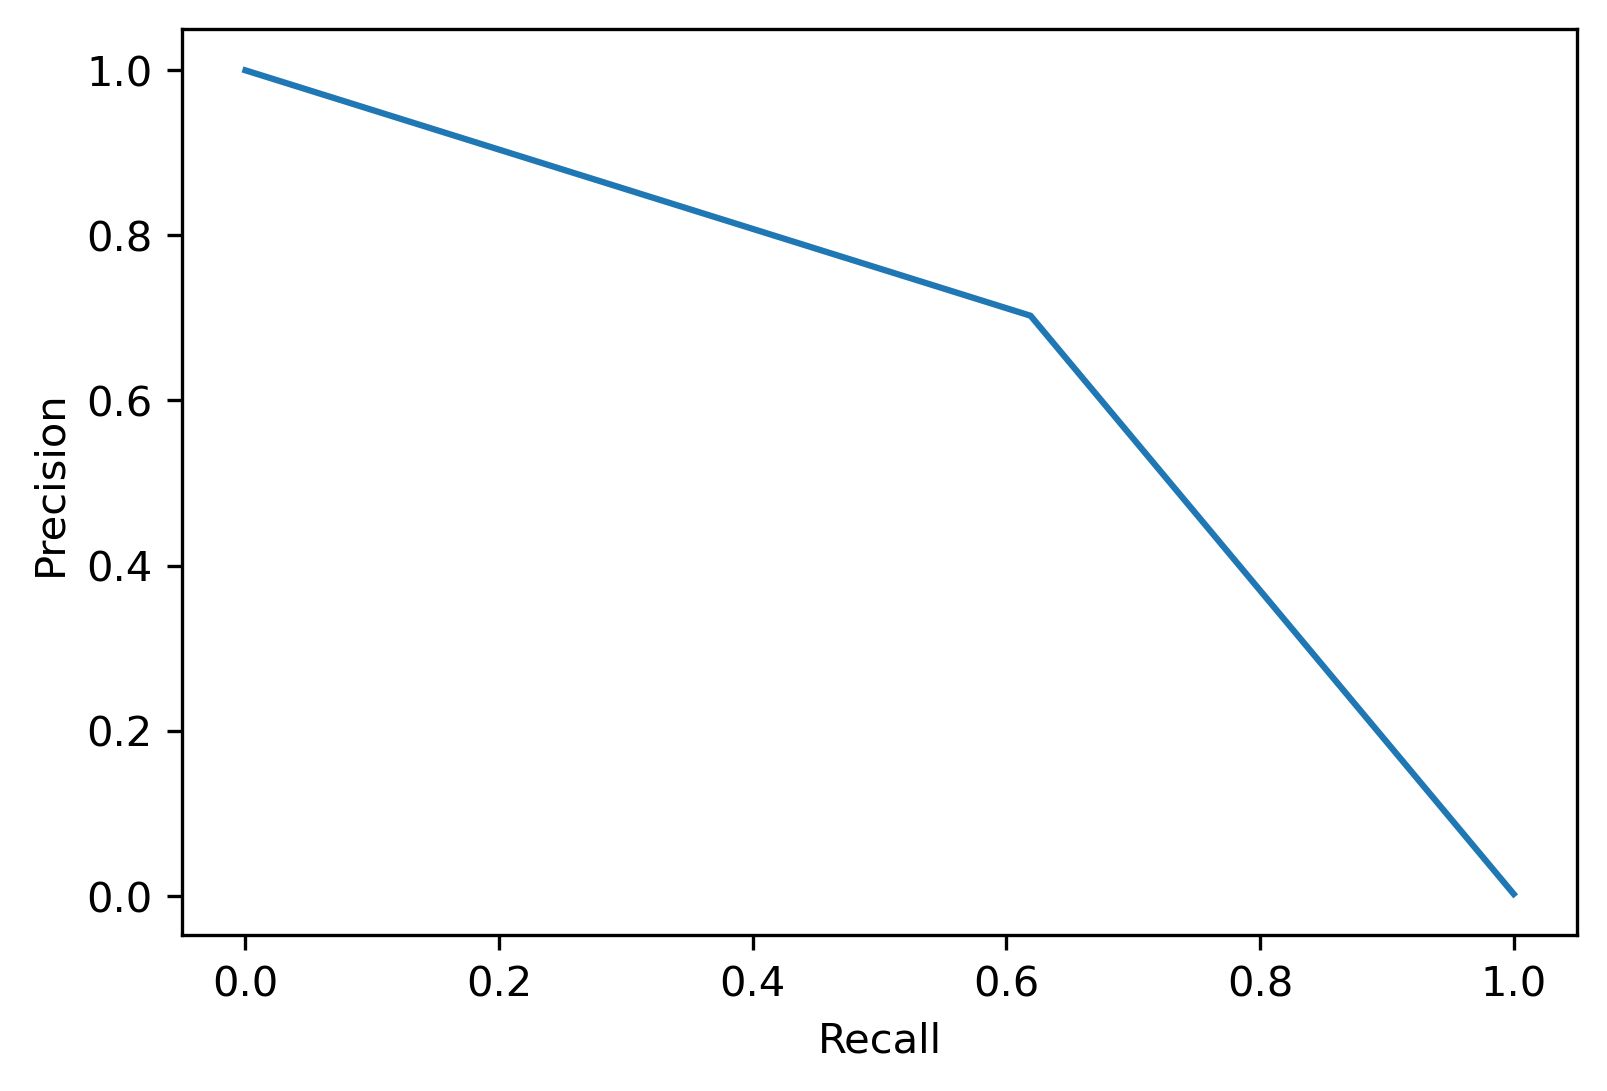
\includegraphics[width=\textwidth]{./images/rfc_prc.png}
    \caption{PRC for Random Forest Classifier. AUC = 0.4358}
    \label{fig:rfc_prc}
  \end{subfigure}
  \caption{ROC and PRC curves}
  \label{fig:roc_and_prc}
\end{figure}

Using the F1 score to compare the models, we find, that the Support Vector Machine is performing best ($F1 = 0.8378$). On the second and third place we have the Random Forest Classifier ($F1 = 0.6582$) and the Logistic Regression with $F1 = 0.6582$. They have exactly the same confusion matrix. Sadly the deep neural network performs worst with an F1 score of only $F1 = 0.6329$, though not much worse than the other methods. This is unexpected and is likely due to not enough data that is available in the fraud-class to have really good training.

\subsection{Performing Undersampling}

I used undersampling to bring the number of non-fraud cases in the train data down to the number of fraud cases. The train set contained 181 fraud cases, so the undersampled train data set now contains, 362 objects in total, half of which are fraud. SVM, Random Forst Classifier and Logistic Regression were trained again on this data. Also the deep neural network was trained on the undersampled data, though with a few modifications to the model proposed in the preceding section.
Because we now have much less training examples we need to bump the number of epochs (from 50 to 2000) to get a similar amount of training work done. Also the batch size was chosen to be slightly lower (32 instead of 64). Still the network has 4 hidden layers with 8 neurons each. The learning rate also stayed 0.0001.

Figure~\ref{fig:u_comp} aims to compare the test-set performance of the 4 models that used undersampling when training.

\begin{figure}[htb]
  \centering
  \begin{subfigure}[b]{0.48\textwidth}
    \centering
    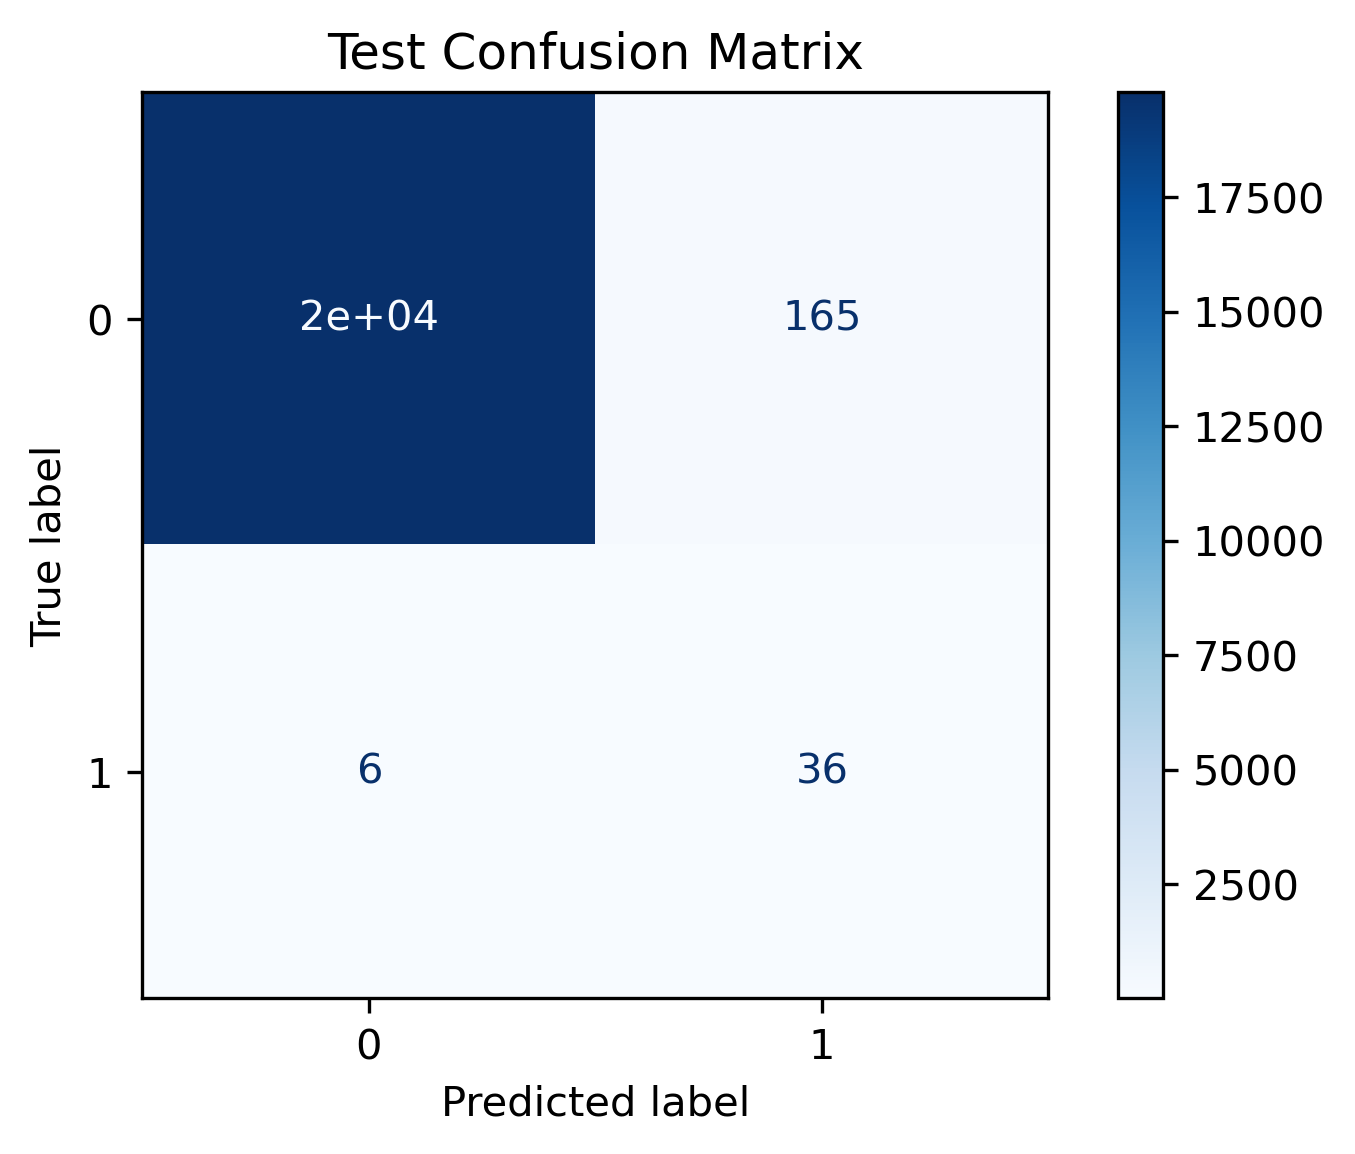
\includegraphics[width=\textwidth]{./images/undersampled_net(d4_k8)_E2000_LR0.0001_B32/conf_test.png}
    \caption{Deep Neural Network}
    \label{fig:u_1}
  \end{subfigure}
  \begin{subfigure}[b]{0.48\textwidth}
    \centering
    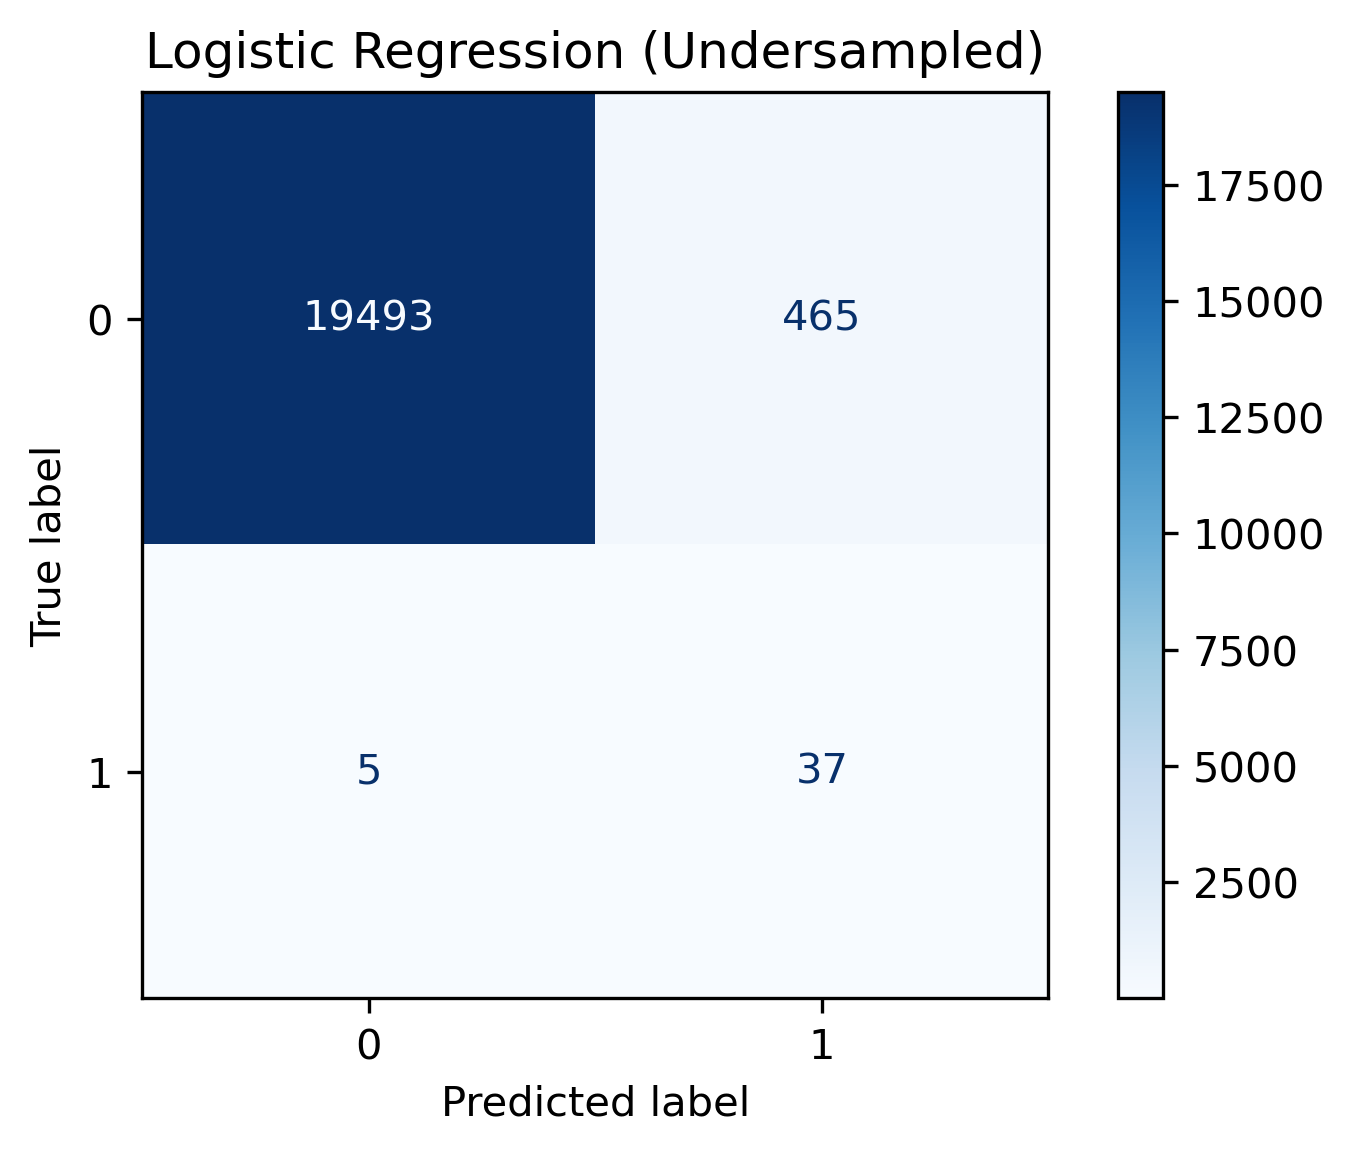
\includegraphics[width=\textwidth]{./images/reg_conf1_u.png}
    \caption{Logistic Regression}
    \label{fig:u2}
  \end{subfigure}
  \begin{subfigure}[b]{0.48\textwidth}
    \centering
    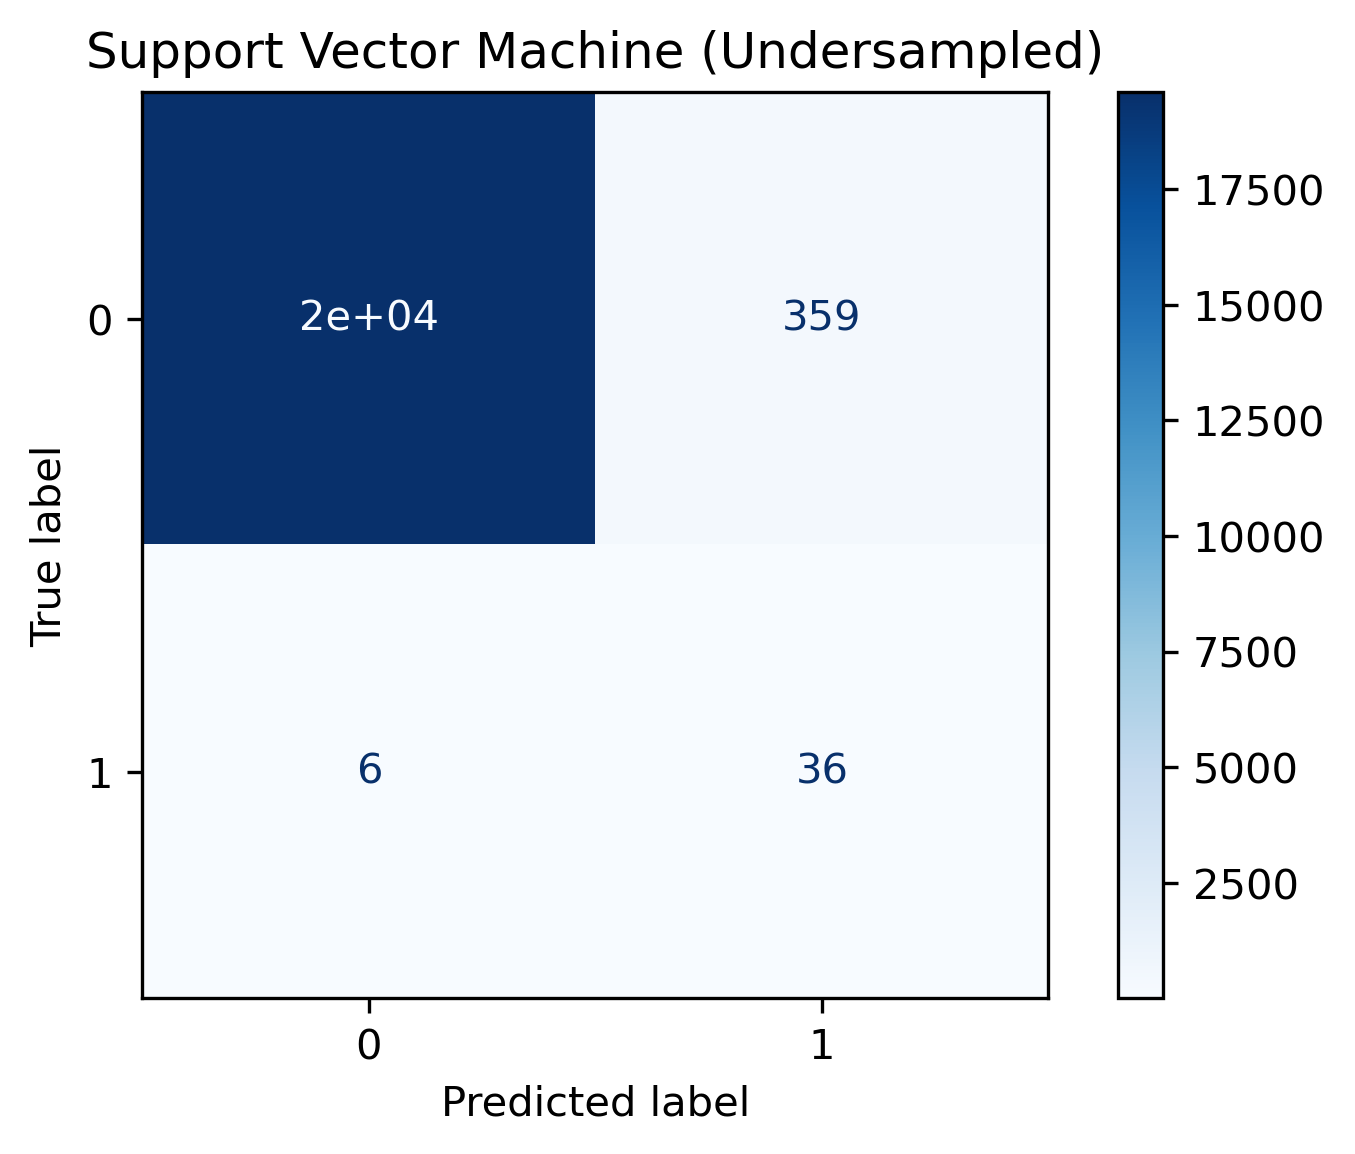
\includegraphics[width=\textwidth]{./images/svm_conf1_u.png}
    \caption{Support Vector Machine}
    \label{fig:u3}
  \end{subfigure}
  \begin{subfigure}[b]{0.48\textwidth}
    \centering
    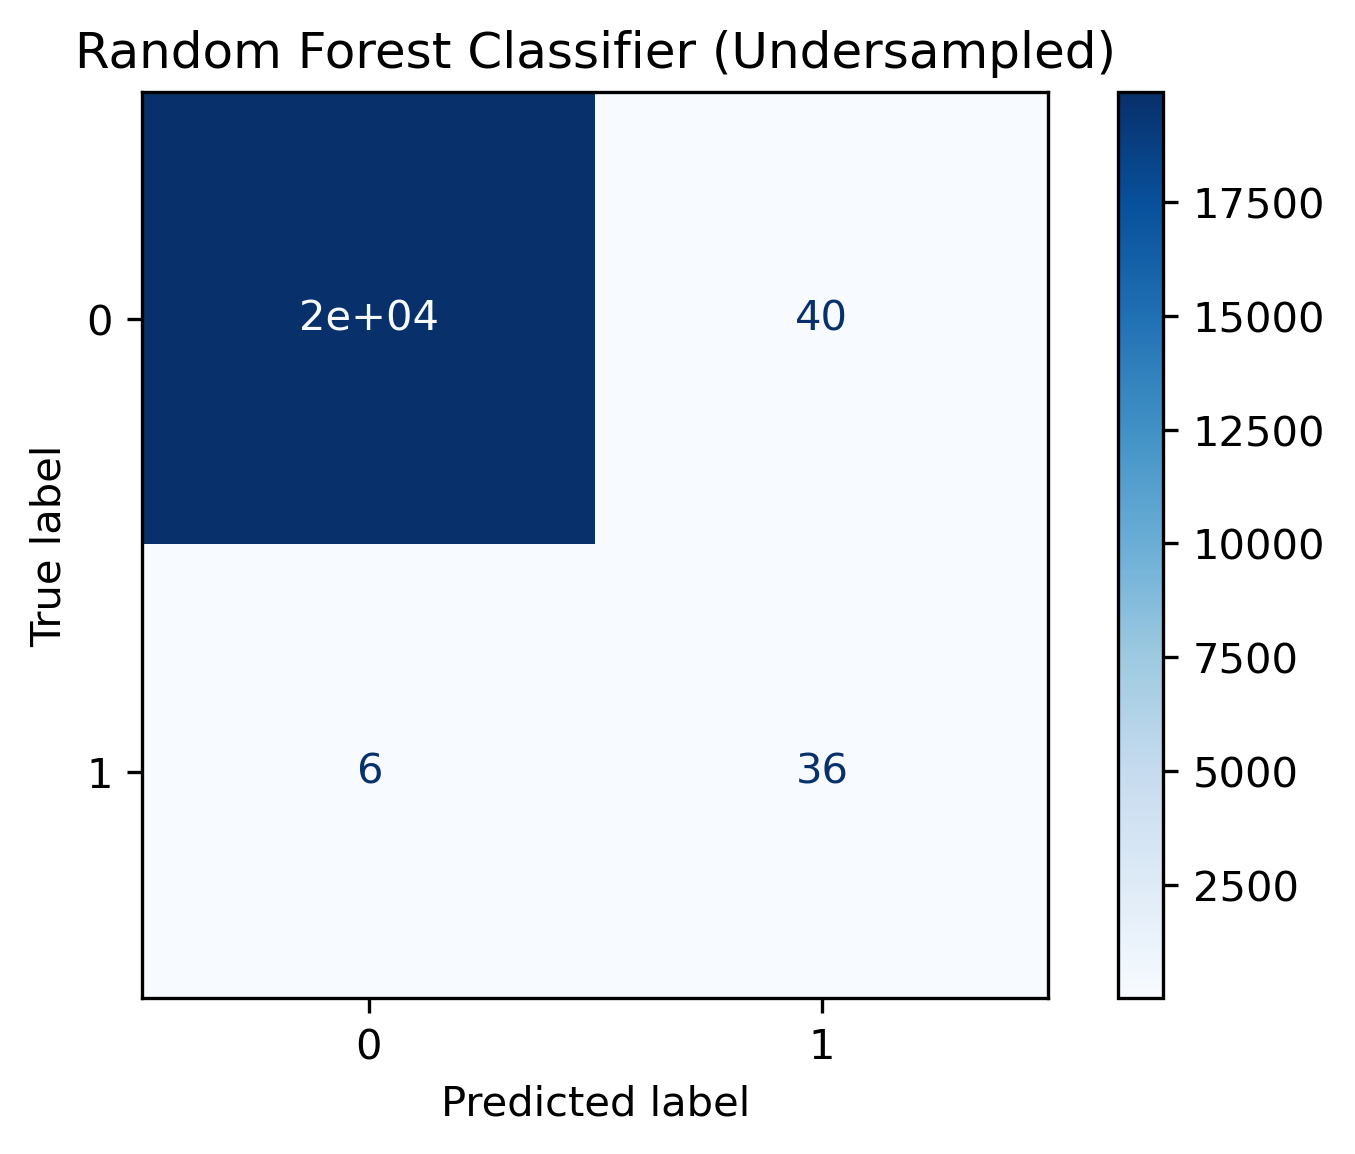
\includegraphics[width=\textwidth]{./images/rfc_conf1_u.png}
    \caption{Random Forest Classifier}
    \label{fig:u4}
  \end{subfigure}
  \caption{Confusion Matrices after Undersampling}
  \label{fig:u_comp}
\end{figure}

At first we can see that a lot more items get misclassified than without undersampling. This can be partly because the train set was massively reduced in size and does not contain so much information to learn from anymore. Especially there are much more False-Positives now. Let's take a look at the actual performance values in Table~\ref{tab:undersampling}. Looking at the F1 score, we can see that all models perform worse than before. The Random Forest Classifier seems to have the least trouble though. However, it is not clear if the performance is really worse. Looking at the Recall, we can see that
all models have improvemed at the cost of precision. For detecting credit card fraud it is probably much more important to catch all true positives (fraud cases) even at the cost of some false alarms (false positives). So it depends on the application if the undersampling makes for better or worse classifiers. The deep neural network can deal with the data now much better than Logistic Regression and the Support Vector Machine and is on second place in terms of the F1-score.

\begin{table}[ht]
  \centering
  \caption{Performance on test set using an undersampled train set}
  \label{tab:undersampling}
  \begin{tabular}{c|cccc}
    characteristic           & Accuracy & Precision   & Recall & F1          \\
    \hline
    Deep Neural Network      & 0.9915   & 0.1791      & 0.8571 & 0.2963      \\
    Logistic Regression      & 0.9765   & 0.0737      & 0.8810 & 0.1360      \\
    Support Vector Machine   & 0.98175  & 0.091139241 & 0.8571 & 0.164759725 \\
    Random Forest Classifier & 0.9977   & 0.473684211 & 0.8571 & 0.610169492 \\
  \end{tabular}
\end{table}


\section{Other ideas for the unbalanced data problem}

Since out of our 99999 objects in the dataset only 223 represent fraud, we need to deal with the unbalanced data in a smart way.
We can use under- or oversampling. However there are also other approaches.

\subsection{Clustering the Majority Class}
Instead of using undersampling, we could also cluster the majority class objects into $n$ clusters, where $n$ is the number of objects in the minority class and use the resulting cluster centers as "examples" for the majority class in training. This way we have a balanced and relatively small dataset but still capture some information from each object from the original data, since each object has some influence on the resulting cluster centers.

\subsection{Stronger Weights for Minority Class}

since there are so few fraud cases, it is easy for a machine learning algorithm to simple oversee them, and not recognize their influence. To avoid this, we could give a greater punishment to the misclassification of fraud cases and in this way force the model to consider them more strongly. We could do this by having an asymmetric loss function, which is steeper in the area where the fraud class would be misclassified.


\section{Discussion}

In total it was surprising that the deep neural network did not outperform the other methods. This could be in part due to not enough information, because the set of fraud cases was so small. Also maybe the wrong architecture or parameters were chosen, but I did my best to try many different values when choosing the best model.

% \newpage
% \addcontentsline{toc}{section}{Bibliography}
% \renewcommand\refname{Bibliography}
% \bibliographystyle{plainnat}
% \bibliography{references}
\end{document}
